\documentclass[12pt, twoside]{article}
\usepackage{amsmath}
\usepackage{amssymb}
\usepackage[colorlinks=true, linkcolor=black]{hyperref} % Links
\usepackage{makeidx} % Indexierung
\usepackage{siunitx}
\usepackage[english]{babel} % deutsche Sonderzeichen
\usepackage[utf8]{inputenc}
\usepackage{geometry} % Dokumentendesign wie Seiten- oder Zeilenabstand bestimmen
\usepackage[toc,page]{appendix}

% Graphiken
\usepackage{tikz}
\usepackage{pgfplots}
\usepackage{pgfcore}
\usepackage{pgfopts}
\usepackage{pgfornament}
\usepackage{pgf}
\usepackage{ifthen}
\usepackage{booktabs}

% Tabellen
\usepackage{tabu}
\usepackage{longtable}
\usepackage{colortbl} % Tabellen faerben
\usepackage{multirow}
\usepackage{diagbox} % Tabellenzelle diagonal splitten

\usepackage{xcolor} % Farben
\usepackage[framemethod=tikz]{mdframed} % Hintergrunderstellung
\usepackage{enumitem} % Enumerate mit Buchstaben nummerierbar machen
\usepackage{pdfpages}
\usepackage{listings} % Source-Code darstellen
\usepackage{eurosym} % Eurosymbol
\usepackage[square,numbers]{natbib}
\usepackage{here} % figure an richtiger Stelle positionieren
\usepackage{verbatim} % Blockkommentare mit \begin{comment}...\end{comment}
\usepackage{ulem} % \sout{} (durchgestrichener Text)

% BibLaTex
\bibliographystyle{acm}

% Aendern des Anhangnamens (Seite und Inhaltsverzeichnis)
%\renewcommand\appendixtocname{Anhang}
%\renewcommand\appendixpagename{Anhang}

% mdframed Style
\mdfdefinestyle{codebox}{
	linewidth=2.5pt,
	linecolor=codebordercolor,
	backgroundcolor=codecolor,
	shadow=true,
	shadowcolor=black!40!white,
	fontcolor=black,
	everyline=true,
}

% Seitenabstaende
\geometry{left=15mm,right=15mm,top=15mm,bottom=20mm}

% TikZ Bibliotheken
\usetikzlibrary{
    arrows,
    arrows.meta,
    decorations,
    backgrounds,
    positioning,
    fit,
    petri,
    shadows,
    datavisualization.formats.functions,
    calc,
    shapes,
    shapes.multipart
}

\pgfplotsset{width=7cm,compat=1.15}

\definecolor{codecolor}{HTML}{EEEEEE}
\definecolor{codebordercolor}{HTML}{CCCCCC}

% Standardeinstellungen fuer Source-Code
\lstset{
    language=C,
    breaklines=true,
    keepspaces=true,
    keywordstyle=\bfseries\color{green!70!black},
    basicstyle=\ttfamily\color{black},
    commentstyle=\itshape\color{purple},
    identifierstyle=\color{blue},
    stringstyle=\color{orange},
    showstringspaces=false,
    rulecolor=\color{black},
    tabsize=2,
    escapeinside={\%*}{*\%},
}

%
% Tikz-library for UML
%

% Arrow tips {{{

  % umlaggreg {{{
  \tikzset{
    umlaggreg /.tip = {Diamond[fill=white,scale=1.75]}
  }
  % }}}

  % umlcompo {{{
  \tikzset{
    umlcompo /.tip = {Diamond[fill=black,scale=1.75]}
  }
  % }}}

  % umlgeneral {{{
  \tikzset{
    umlgeneral /.tip = {Triangle[fill=white,scale=1.75]}
  }
  % }}}

  % umlportprovider {{{
  \tikzset{
    umlportprovider /.tip = {Circle[
      length=8pt,
      width=8pt,
      fill=white
    ]}
  }
  % }}}

  % umlportproviderREST {{{
  \tikzset{
    umlportproviderREST /.tip = {Circle[
      length=8pt,
      width=8pt,
      fill=blue
    ]}
  }
  % }}}

  % umlportproviderEvent {{{
  \tikzset{
    umlportproviderEvent /.tip = {Circle[
      length=8pt,
      width=8pt,
      fill=red
    ]}
  }
  % }}}

  % umlportcaller {{{
  \tikzset{
    umlportcaller /.tip = {Arc Barb[
      reversed,
      length=3pt,
      width=8pt
    ]}
  }
  % }}}

% }}}

% Use-case {{{
\tikzset{
  usecase/.style={
    ellipse,
    fill=blue!20,
    align=center,
    draw
  }
}
% }}}

%%%%%%%%%%%%%%%%%%%%%%%%%%%%%%%%%%%%%%%%%%%%%%%%%%%%%%%%%%%%%%%%%%%%%%%%%%%%%%%%%%%%%%%%%%%%%%%%%%%%%%%%%%%%%%%%%%%%%%%%%%%%%%%%%%%%%%%%%%%%%%%%%%
%UML Component Token
%%%%%%%%%%%%%%%%%%%%%%%%%%%%%%%%%%%%%%%%%%%%%%%%%%%%%%%%%%%%%%%%%%%%%%%%%%%%%%%%%%%%%%%%%%%%%%%%%%%%%%%%%%%%%%%%%%%%%%%%%%%%%%%%%%%%%%%%%%%%%%%%%%
\def\UMLComponentToken#1#2#3{
	\draw [#3]($(#1.north east)-(0.1,0.1)$) rectangle ($(#1.north east)-(0.3,0.45)$);
	\draw [#3,fill=#2]($(#1.north east)-(0.35,0.2)$) rectangle ($(#1.north east)-(0.25,0.25)$);
	\draw [#3,fill=#2]($(#1.north east)-(0.35,0.3)$) rectangle ($(#1.north east)-(0.25,0.35)$);
}

%%%%%%%%%%%%%%%%%%%%%%%%%%%%%%%%%%%%%%%%%%%%%%%%%%%%%%%%%%%%%%%%%%%%%%%%%%%%%%%%%%%%%%%%%%%%%%%%%%%%%%%%%%%%%%%%%%%%%%%%%%%%%%%%%%%%%%%%%%%%%%%%%%
%UML Component
%%%%%%%%%%%%%%%%%%%%%%%%%%%%%%%%%%%%%%%%%%%%%%%%%%%%%%%%%%%%%%%%%%%%%%%%%%%%%%%%%%%%%%%%%%%%%%%%%%%%%%%%%%%%%%%%%%%%%%%%%%%%%%%%%%%%%%%%%%%%%%%%%%
%USAGE:
% 	\UMLComponent{name}{width}{height}{Position eines Ports und Beschreibender UMLNote in der Form:
%																				positionPort/noteX/noteY/noteText/noteColor
%
%BEISPIEL:
%		\UMLComponent{Bestellvorgang}{\linewidth-0.2cm}{15cm}{
%			Bestellvorgang.east/7/1.5/Bestellvorgang ausf\"uhren/yellow!25,
%			Bestellvorgang.south/-2/-6/Blah/yellow!25,
%			Bestellvorgang.310/7/-6/Blahhh/yellow!25
%		}
\def\UMLComponent#1#2#3#4{
	\node [rectangle split, rectangle split parts = 2,rectangle split empty part height=#3,draw,fill=yellow!25,inner ysep=7pt,inner xsep=15pt,minimum size=#2] at(0,0) (#1) {#1 \nodepart{second}};
	\UMLComponentToken{#1}{yellow!25}{}
	\foreach \port/\notex/\notey/\notetext/\notecolor in {#4}{
		\UMLNote{\notex}{\notey}{\notetext}{\port}{\notecolor};
		\draw[fill=yellow!25] ($(\port) - (.2,.2)$) rectangle ($(\port)+(.2,.2)$);
	};
}

% UML Simple Component {{{

% 1. x
% 2. y
% 3. text/name
% 4. options
\def\UMLSComponent#1#2#3#4{
	\node[
    rectangle split,
    rectangle split parts = 2,
    rectangle split empty part height=1cm,
    draw,
    fill=yellow!25,
    inner ysep=7pt,
    inner xsep=15pt,
    #4
  ] at(#1,#2) (#3) {#3 \nodepart{second}};
	\UMLComponentToken{#3}{yellow!25}{}
}

% 1. Relative to
% 2. Text/Name
% 3. Options
\def\UMLSComponentRelativeTo#1#2#3{
	\node[
    rectangle split,
    rectangle split parts = 2,
    rectangle split empty part height=1cm,
    draw,
    fill=yellow!25,
    inner ysep=7pt,
    inner xsep=15pt,
    #1,
    #3
  ] (#2) {#2 \nodepart{second}};
	\UMLComponentToken{#2}{yellow!25}{}
}

% 1. Relative to
% 2. Text
% 3. Name
% 4. Options
\def\UMLSComponentRelativeToAlterName#1#2#3#4{
	\node[
    rectangle split,
    rectangle split parts = 2,
    rectangle split empty part height=1cm,
    draw,
    fill=yellow!25,
    inner ysep=7pt,
    inner xsep=15pt,
    #1,
    #4
  ] (#3) {#2 \nodepart{second}};
	\UMLComponentToken{#3}{yellow!25}{}
}

% 1. Relative to
% 2. Text
% 3. Name
% 4. Options
\def\UMLSComponentRelativeToAlterName#1#2#3#4{
	\node [rectangle split, rectangle split parts = 2,rectangle split empty part height=1cm,draw, fill=yellow!25,inner ysep=7pt,inner xsep=15pt,#1,#4](#3) {#2 \nodepart{second}};
	\UMLComponentToken{#3}{yellow!25}{}
}

% }}}

%%%%%%%%%%%%%%%%%%%%%%%%%%%%%%%%%%%%%%%%%%%%%%%%%%%%%%%%%%%%%%%%%%%%%%%%%%%%%%%%%%%%%%%%%%%%%%%%%%%%%%%%%%%%%%%%%%%%%%%%%%%%%%%%%%%%%%%%%%%%%%%%%%
%UML Extern Component
%%%%%%%%%%%%%%%%%%%%%%%%%%%%%%%%%%%%%%%%%%%%%%%%%%%%%%%%%%%%%%%%%%%%%%%%%%%%%%%%%%%%%%%%%%%%%%%%%%%%%%%%%%%%%%%%%%%%%%%%%%%%%%%%%%%%%%%%%%%%%%%%%%
\def\UMLExternComponent#1#2#3{
	\node [rectangle split, rectangle split parts = 2,rectangle split empty part height=1cm,draw, fill=black!10,inner ysep=7pt,inner xsep=15pt] at(#1,#2) (#3) {$<<$#3$>>$ \nodepart{second}};
	\UMLComponentToken{#3}{black!10}{}
}

%%%%%%%%%%%%%%%%%%%%%%%%%%%%%%%%%%%%%%%%%%%%%%%%%%%%%%%%%%%%%%%%%%%%%%%%%%%%%%%%%%%%%%%%%%%%%%%%%%%%%%%%%%%%%%%%%%%%%%%%%%%%%%%%%%%%%%%%%%%%%%%%%%
%UML Note
%%%%%%%%%%%%%%%%%%%%%%%%%%%%%%%%%%%%%%%%%%%%%%%%%%%%%%%%%%%%%%%%%%%%%%%%%%%%%%%%%%%%%%%%%%%%%%%%%%%%%%%%%%%%%%%%%%%%%%%%%%%%%%%%%%%%%%%%%%%%%%%%%%
%USAGE:
%	\UMLNote{x}{y}{text}{to (--)}{color (rectangle north east)}
\def\UMLNote#1#2#3#4#5{
	\node [rectangle,fill=green!25,draw,inner ysep=15pt,inner xsep=6pt,text width=3cm] at (#1,#2) (b) {\small{#3}};
	\draw [fill=#5,#5]($(b.north east) + (.1,.1)$) -- ($(b.north east) - (0,.5)$) -- ($(b.north east) - (.5,0)$) -- cycle;
	\draw ($(b.north east) - (.01,.5)$) -- ($(b.north east) - (.5,.01)$) -- ($(b.north east)-(.5,.5)$) -- cycle;
	\draw [dashed](b) -- (#4);
}

%%%%%%%%%%%%%%%%%%%%%%%%%%%%%%%%%%%%%%%%%%%%%%%%%%%%%%%%%%%%%%%%%%%%%%%%%%%%%%%%%%%%%%%%%%%%%%%%%%%%%%%%%%%%%%%%%%%%%%%%%%%%%%%%%%%%%%%%%%%%%%%%%%
% UML Component Port
%%%%%%%%%%%%%%%%%%%%%%%%%%%%%%%%%%%%%%%%%%%%%%%%%%%%%%%%%%%%%%%%%%%%%%%%%%%%%%%%%%%%%%%%%%%%%%%%%%%%%%%%%%%%%%%%%%%%%%%%%%%%%%%%%%%%%%%%%%%%%%%%%%

% 1. position
% 2. options (draw)
\def\UMLComponentPort#1#2{
	\draw[fill=yellow!25,#2] ($(#1)-(.2,.2)$) rectangle ($(#1)+(.2,.2)$);
}

%%%%%%%%%%%%%%%%%%%%%%%%%%%%%%%%%%%%%%%%%%%%%%%%%%%%%%%%%%%%%%%%%%%%%%%%%%%%%%%%%%%%%%%%%%%%%%%%%%%%%%%%%%%%%%%%%%%%%%%%%%%%%%%%%%%%%%%%%%%%%%%%%%
% UML Component Connector with Ports on both ends
%%%%%%%%%%%%%%%%%%%%%%%%%%%%%%%%%%%%%%%%%%%%%%%%%%%%%%%%%%%%%%%%%%%%%%%%%%%%%%%%%%%%%%%%%%%%%%%%%%%%%%%%%%%%%%%%%%%%%%%%%%%%%%%%%%%%%%%%%%%%%%%%%%
\def\UMLComponentPortConnector#1#2#3#4#5#6#7#8{
	\draw[#3,-{>[sep=3.5]>}] (#1) #4 (#2);
	\UMLNote{#5}{#6}{#7}{#2}{#8}
	\draw[fill=yellow!25] ($(#1)-(.2,.2)$) rectangle ($(#1)+(.2,.2)$);
	\draw[fill=yellow!25] ($(#2)-(.2,.2)$) rectangle ($(#2)+(.2,.2)$);
}

%%%%%%%%%%%%%%%%%%%%%%%%%%%%%%%%%%%%%%%%%%%%%%%%%%%%%%%%%%%%%%%%%%%%%%%%%%%%%%%%%%%%%%%%%%%%%%%%%%%%%%%%%%%%%%%%%%%%%%%%%%%%%%%%%%%%%%%%%%%%%%%%%%
% UML Component Realizor with Ports on both ends
%%%%%%%%%%%%%%%%%%%%%%%%%%%%%%%%%%%%%%%%%%%%%%%%%%%%%%%%%%%%%%%%%%%%%%%%%%%%%%%%%%%%%%%%%%%%%%%%%%%%%%%%%%%%%%%%%%%%%%%%%%%%%%%%%%%%%%%%%%%%%%%%%%
\def\UMLComponentPortRealizor#1#2#3#4#5#6#7#8{
	\draw[#3,-{Stealth[sep=3.5,inset=0pt,length=5pt,width=5pt]>},blue] (#1) #4 (#2);
	\UMLNote{#5}{#6}{#7}{#2}{#8}
	\draw[fill=yellow!25] ($(#1)-(.2,.2)$) rectangle ($(#1)+(.2,.2)$);
	\draw[fill=yellow!25] ($(#2)-(.2,.2)$) rectangle ($(#2)+(.2,.2)$);
}

% UML Class (various) {{{
%
% 1. Normal                         -> \UMLClass { X } { Y } { Text/Name } { Options (node) }
% 2. Normal mit alternativem Namen  -> \UMLClassAlterName { X } { Y } { Text } { Name } { Options (node) }
% 3. Relativ                        -> \UMLClassRelativeTo { Relative to } { Text/Name } { Options (node) }
% 4. Relativ mit alternativem Namen -> \UMLClassRelativeToAlterName { Relative to } { Text } { Name } { Options (node) }

  % 1. Normal {{{
  \def\UMLClass#1#2#3#4{
    \node [
      fill = yellow!25,
      rectangle split,
      rectangle split parts = 3,
      rectangle split ignore empty parts = true,
      rectangle split part align = {center, left, left},
      inner xsep = 15pt,
      inner ysep = 7pt,
      draw,
      #4
    ] at(#1,#2) (#3) {#3};
  }
  % }}}

  % 2. Normal mit alternativem Namen {{{
    \def\UMLClassAlterName#1#2#3#4#5{
      \node [
        fill = yellow!25,
        rectangle split,
        rectangle split parts = 3,
        rectangle split ignore empty parts = true,
        rectangle split part align = {center, left, left},
        inner xsep = 15pt,
        inner ysep = 7pt,
        draw,
        #5
      ] at (#1, #2) (#4) {#3};
    }
  % }}}

  % 3. Relativ {{{
    \def\UMLClassRelativeTo#1#2#3{
      \node [
        fill = yellow!25,
        rectangle split,
        rectangle split parts = 3,
        rectangle split ignore empty parts = true,
        rectangle split part align = {center, left, left},
        inner xsep = 15pt,
        inner ysep = 7pt,
        draw,
        #1,
        #3
      ] (#2) {#2};
    }
  % }}}

  % 4. Relativ {{{
    \def\UMLClassRelativeToAlterName#1#2#3#4{
      \node [
        fill = yellow!25,
        rectangle split,
        rectangle split parts = 3,
        rectangle split ignore empty parts = true,
        rectangle split part align = {center, left, left},
        inner xsep = 15pt,
        inner ysep = 7pt,
        draw,
        #1,
        #4
      ] (#3) {#2};
    }
  % }}}

% }}}

% UML Actor (various) {{{
%
% 1. Normal
%    -> \UMLActor { X } { Y } { Text/Name }
% 2. Normal mit alternativem Namen
%    -> \UMLActorAlterName { X } { Y } { Text } { Name }
% 3. Relativ
%    -> \UMLActorRelativeTo { Relative to } { Text/Name }
% 4. Relativ mit alternativem Namen
%    -> \UMLActorRelativeToAlterName { Relative to } { Text } { Name }

  % DrawActor {{{
  \def\DrawActor#1{

    % Body {{{
    \draw[scale=.5] ($(#1)+(0,.5)$) -- ($(#1)-(0,.5)$);
    % }}}

    % Left leg {{{
    \draw[scale=.5] ($(#1)-(0,.5)$) -- ($(#1)+(.5,-1)$);
    % }}}

    % Right leg {{{
    \draw[scale=.5] ($(#1)-(0,.5)$) -- ($(#1)+(-.5,-1)$);
    % }}}

    % Arms {{{
    \draw[scale=.5] ($(#1)+(.5,.25)$) -- ($(#1)+(-.5,.25)$);
    % }}}

    % Head {{{
    \draw[scale=.5] ($(#1)+(0,.75)$) circle (.25);
    % }}}

  }
  % }}}

  % 1. Normal {{{
  \def\UMLActor#1#2#3{

    % Node for referencing actor {{{
    \node[
      label=below:#3,
      inner ysep=.55cm,
      inner xsep=.3cm
    ] at (#1,#2) (#3) {};
    % }}}

    \DrawActor{#3}

  }
  % }}}

  % 2. Normal mit alternativem Namen {{{
  \def\UMLActorAlterName#1#2#3#4{

    % Node for referencing actor {{{
    \node[
      label=below:#3,
      inner ysep=.55cm,
      inner xsep=.3cm
    ] at (#1,#2) (#4) {};
    % }}}

    \DrawActor{#4}

  }
  % }}}

  % 3. Relativ {{{
  \def\UMLActorRelativeTo#1#2{

    % Node for referencing actor {{{
    \node[
      label=below:#2,
      inner ysep=.55cm,
      inner xsep=.3cm,
      #1
    ] (#2) {};
    % }}}

    \DrawActor{#2}

  }
  % }}}

  % 4. Relativ {{{
  \def\UMLActorRelativeToAlterName#1#2#3{

    % Node for referencing actor {{{
    \node[
      label=below:#2,
      inner ysep=.55cm,
      inner xsep=.3cm,
      #1
    ] (#3) {};
    % }}}

    \DrawActor{#3}

  }
  % }}}

% }}}

%
% UML Activity State (various)
%
% 1. Normal                         -> \UMLActivityState{ X }{ Y }{ Text/Name }{ Options (node) }
% 2. Normal mit alternativem Namen  -> \UMLActivityStateAlterName{ X }{ Y }{ Text }{ Name }{ Options (node) }
% 3. Relativ                        -> \UMLActivityStateRelativeTo{ Relative to }{ Text/Name }{ Options (node) }
% 4. Relativ mit alternativem Namen -> \UMLActivityStateRelativeToAlterName{ Relative to }{ Text }{ Name }{ Options (node) }
%
%

% 1. Normal
%
% #1: X
% #2: Y
% #3: Text/Name
% #4: Options (node)

\def\UMLActivityState#1#2#3#4{
	\node [rectangle,rounded corners,draw,fill=black!10,inner ysep=9pt,inner xsep=22pt,#4] at(#1,#2) (#3) {#3};
	\UMLActivityStateToken{#3}
}

% 2. Alternativer Name
%
% #1: X
% #2: Y
% #3: Text
% #4: Name
% #5: Options (node)

\def\UMLActivityStateAlterName#1#2#3#4#5{
	\node [rectangle,rounded corners,draw,fill=black!10,inner ysep=9pt,inner xsep=22pt,#5] at(#1,#2) (#4) {#3};
	\UMLActivityStateToken{#4}
}


% 3. Relativ
%
% #1: Relative to (z.B. below=1 of ...)
% #2: Text/Name
% #3: Options (node)

\def\UMLActivityStateRelativeTo#1#2#3{
	\node [rectangle,rounded corners,draw,fill=black!10,inner ysep=9pt,inner xsep=22pt,#1,#3] (#2) {#2};
	\UMLActivityStateToken{#2}
}


% 4. Relativ mit alternativem Namen
%
% #1: Relative to (z.B. below=1 of ...)
% #2: Text
% #3: Name
% #4: Options

\def\UMLActivityStateRelativeToAlterName#1#2#3#4{
	\node [rectangle,rounded corners,draw,fill=black!10,inner ysep=9pt,inner xsep=22pt,#1,#4] (#3) {#2};
	\UMLActivityStateToken{#3}
}


% Token

\def\UMLActivityStateToken#1{
	\draw[fill=yellow!25,rounded corners] ($(#1.west)+(.3,.25)$) rectangle ($(#1.west)+(.7,-.15)$);
}


%
% UML Activity Object (various)
%
% 1. Normal                         -> \UMLActivityObject{ X }{ Y }{ Text/Name }{ Options (node) }
% 2. Normal mit alternativem Namen  -> \UMLActivityObjectAlterName{ X }{ Y }{ Text }{ Name }{ Options (node) }
% 3. Relativ                        -> \UMLActivityObjectRelativeTo{ Relative to }{ Text/Name }{ Options (node) }
% 4. Relativ mit alternativem Namen -> \UMLActivityObjectRelativeToAlterName{ Relative to }{ Text }{ Name }{ Options (node) }
%
%

% 1. Normal
%
% #1: X
% #2: Y
% #3: Text/Name
% #4: Options (node)

\def\UMLActivityObject#1#2#3#4{
	\node [rectangle,draw,fill=green!15,inner ysep=9pt,inner xsep=25pt,#4] at(#1,#2) (#3) {:#3};
	\UMLActivityObjectToken{#3}
}


% 2. Alternativer Name
%
% #1: X
% #2: Y
% #3: Text
% #4: Name
% #5: Options (node)

\def\UMLActivityObjectAlterName#1#2#3#4#5{
	\node [rectangle,draw,fill=green!15,inner ysep=9pt,inner xsep=25pt,#5] at(#1,#2) (#4) {:#3};
	\UMLActivityObjectToken{#4}
}


% 3. Relativ
%
% #1: Relative to (z.B. below=1 of ...)
% #2: Text/Name
% #3: Options (node)

\def\UMLActivityObjectRelativeTo#1#2#3{
	\node [rectangle,draw,fill=green!15,inner ysep=9pt,inner xsep=25pt,#3,#1] (#2) {:#2};
	\UMLActivityObjectToken{#2}
}


% 4. Relativ mit alternativem Namen
%
% #1: Relative to (z.B. below=1 of ...)
% #2: Text
% #3: Name
% #4: Options

\def\UMLActivityObjectRelativeToAlterName#1#2#3#4{
	\node [rectangle,draw,fill=green!15,inner ysep=9pt,inner xsep=25pt,#4,#1] (#3) {:#2};
	\UMLActivityObjectToken{#3}
}


% Token

\def\UMLActivityObjectToken#1{
	\draw[fill=yellow!25] ($(#1.west)+(.3,.25)$) rectangle ($(#1.west)+(.7,.11)$);
	\draw ($(#1.west)+(.35,.18)$) -- ($(#1.west)+(.65,.18)$);
	\draw[fill=yellow!25] ($(#1.west)+(.3,.11)$) rectangle ($(#1.west)+(.7,-.02)$);
	\draw[fill=yellow!25] ($(#1.west)+(.3,-.02)$) rectangle ($(#1.west)+(.7,-.15)$);
}


%
% UML Activity Data Storage (various)
%
% 1. Normal                         -> \UMLActivityDataStorage{ X }{ Y }{ Text/Name }{ Options (node) }
% 2. Normal mit alternativem Namen  -> \UMLActivityDataStorageAlterName{ X }{ Y }{ Text }{ Name }{ Options (node) }
% 3. Relativ                        -> \UMLActivityDataStorageRelativeTo{ Relative to }{ Text/Name }{ Options (node) }
% 4. Relativ mit alternativem Namen -> \UMLActivityDataStorageRelativeToAlterName{ Relative to }{ Text }{ Name }{ Options (node) }
%
%

% 1. Normal
%
% #1: X
% #2: Y
% #3: Text/Name
% #4: Options (node)

\def\UMLActivityDataStorage#1#2#3#4{
	\node [rectangle,draw,fill=green!15,inner ysep=9pt,inner xsep=25pt,#4] at(#1,#2) (#3) {#3};
	\UMLActivityDataStorageToken{#3}
}


% 2. Alternativer Name
%
% #1: X
% #2: Y
% #3: Text
% #4: Name
% #5: Options (node)

\def\UMLActivityDataStorageAlterName#1#2#3#4#5{
	\node [rectangle,draw,fill=green!15,inner ysep=9pt,inner xsep=25pt,#5] at(#1,#2) (#4) {#3};
	\UMLActivityDataStorageToken{#4}
}


% 3. Relativ
%
% #1: Relative to (z.B. below=1 of ...)
% #2: Text/Name
% #3: Options (node)

\def\UMLActivityDataStorageRelativeTo#1#2#3{
	\node [rectangle,draw,fill=green!15,inner ysep=9pt,inner xsep=25pt,#3,#1] (#2) {#2};
	\UMLActivityDataStorageToken{#2}
}


% 4. Relativ mit alternativem Namen
%
% #1: Relative to (z.B. below=1 of ...)
% #2: Text
% #3: Name
% #4: Options

\def\UMLActivityDataStorageRelativeToAlterName#1#2#3#4{
	\node [rectangle,draw,fill=green!15,inner ysep=9pt,inner xsep=25pt,#4,#1] (#3) {#2};
	\UMLActivityDataStorageToken{#3}
}


% Token

\def\UMLActivityDataStorageToken#1{
	\node[rectangle,draw,scale=.5,fill=yellow!25] at($(#1.west)+(.5,-.05)$) (ds) {DS};
	\draw[-{>[scale width=.5]}] ($(ds.north west)+(0,.15)$) -| (ds.north);
	\draw[-{>[scale width=.5]}] (ds.east) -- ($(ds.east)+(.15,0)$);
}


%
% UML Activity Central Buffer (various)
%
% 1. Normal                         -> \UMLActivityCentralBuffer{ X }{ Y }{ Text/Name }{ Options (node) }
% 2. Normal mit alternativem Namen  -> \UMLActivityCentralBufferAlterName{ X }{ Y }{ Text }{ Name }{ Options (node) }
% 3. Relativ                        -> \UMLActivityCentralBufferRelativeTo{ Relative to }{ Text/Name }{ Options (node) }
% 4. Relativ mit alternativem Namen -> \UMLActivityCentralBufferRelativeToAlterName{ Relative to }{ Text }{ Name }{ Options (node) }
%
%

% 1. Normal
%
% #1: X
% #2: Y
% #3: Text/Name
% #4: Options (node)

\def\UMLActivityCentralBuffer#1#2#3#4{
	\node [rectangle,draw,fill=green!15,inner ysep=9pt,inner xsep=25pt,#4] at(#1,#2) (#3) {#3};
	\UMLActivityCentralBufferToken{#3}
}


% 2. Alternativer Name
%
% #1: X
% #2: Y
% #3: Text
% #4: Name
% #5: Options (node)

\def\UMLActivityCentralBufferAlterName#1#2#3#4#5{
	\node [rectangle,draw,fill=green!15,inner ysep=9pt,inner xsep=25pt,#5] at(#1,#2) (#4) {#3};
	\UMLActivityCentralBufferToken{#4}
}


% 3. Relativ
%
% #1: Relative to (z.B. below=1 of ...)
% #2: Text/Name
% #3: Options (node)

\def\UMLActivityCentralBufferRelativeTo#1#2#3{
	\node [rectangle,draw,fill=green!15,inner ysep=9pt,inner xsep=25pt,#3,#1] (#2) {#2};
	\UMLActivityCentralBufferToken{#2}
}


% 4. Relativ mit alternativem Namen
%
% #1: Relative to (z.B. below=1 of ...)
% #2: Text
% #3: Name
% #4: Options

\def\UMLActivityCentralBufferRelativeToAlterName#1#2#3#4{
	\node [rectangle,draw,fill=green!15,inner ysep=9pt,inner xsep=25pt,#4,#1] (#3) {#2};
	\UMLActivityCentralBufferToken{#3}
}


% Token

\def\UMLActivityCentralBufferToken#1{
	\node[rectangle,draw,scale=.5,fill=yellow!25] at($(#1.west)+(.5,-.05)$) (cb) {CB};
	\draw[-{>[scale width=.5]}] ($(cb.north west)+(0,.15)$) -| (cb.north);
	\draw[-{>[scale width=.5]}] (cb.east) -- ($(cb.east)+(.15,0)$);
}


% 1. N1
% 2. N2
% 3. Path
\def\UMLActivityControlFlow#1#2#3{
	\draw[blue,->] (#1) #3 (#2);
}

% 1. N1
% 2. N2
% 3. Path
% 4. Text
% 5. Text Pos
% 6. Text Options
\def\UMLActivityControlFlowWithGuard#1#2#3#4#5#6{
	\draw[blue,->] (#1) #3 (#2);
	\node[#6] at ($(#1)!#5!(#2)$) {\tiny{[#4]}};
}

% 1. N1
% 2. N2
% 3. Path
% 4. Text
% 5. Text Pos
% 6. Text Options
\def\UMLActivityControlFlowWithText#1#2#3#4#5#6{
	\draw[blue,->] (#1) #3 (#2);
	\node[#6] at ($(#1)!#5!(#2)$) {\tiny{#4}};
}



% UML Activity Data Flow (various)

\def\UMLActivityDataFlowPort#1#2#3{
	\draw[fill=#3] ($(#1)-(.15,.15)$) rectangle ($(#1)+(.15,.15)$);
	\draw[->,rotate=#2] ($(#1)-(.1,0)$) -- ($(#1)+(.1,0)$);
}

\def\UMLActivityDataFlow#1#2#3#4#5{
	\draw[brown!50!black,-{>[sep=3pt]>}] (#1) #3 (#2);
	\UMLActivityDataFlowPort{#1}{#4}{blue!25}
	\UMLActivityDataFlowPort{#2}{#5}{orange!25}
}

% 1. N1
% 2. N2
% 3. Path
% 4. Text
% 5. Text Options N1
% 6. Text Options N2
% 7. Arrow Direction (Deg) N1
% 8. Arrow Direction (Deg) N2

\def\UMLActivityDataFlowWithText#1#2#3#4#5#6#7#8{
	\draw[brown!50!black,-{>[sep=3pt]>}] (#1) #3 (#2);
	\node[#5] at (#1) {\tiny{#4}};
	\node[#6] at (#2) {\tiny{#4}};
	\UMLActivityDataFlowPort{#1}{#7}{blue!25}
	\UMLActivityDataFlowPort{#2}{#8}{orange!25}
}

\def\UMLActivityDataFlowNoPorts#1#2#3{
	\draw[brown!50!black,->] (#1) #3 (#2);
}

\def\UMLActivityDataFlowIn#1#2#3#4{
	\draw[brown!50!black,-{>[sep=3pt]>}] (#1) #3 (#2);
	\UMLActivityDataFlowPort{#2}{#4}{orange!25}
}

% 1. N1
% 2. N2
% 3. Path
% 4. Text
% 5. Text Pos
% 6. Text Options
% 7. Arrow Direction (Deg)

\def\UMLActivityDataFlowInWithText#1#2#3#4#5#6#7{
	\draw[brown!50!black,-{>[sep=3pt]>}] (#1) #3 (#2);
	\node[#6] at ($(#1)!#5!(#2)$) {\tiny{#4}};
	\UMLActivityDataFlowPort{#2}{#7}{orange!25}
}

\def\UMLActivityDataFlowOut#1#2#3#4{
	\draw[brown!50!black,->] (#1) #3 (#2);
	\UMLActivityDataFlowPort{#1}{#4}{blue!25}
}

\def\UMLActivityDataFlowOutWithText#1#2#3#4#5#6#7{
	\draw[brown!50!black,->] (#1) #3 (#2);
	\node[#6] at ($(#1)!#5!(#2)$) {\tiny{#4}};
	\UMLActivityDataFlowPort{#1}{#7}{blue!25}
}


% Nodes

\def\UMLActivityInitialNode#1#2{
	\node[circle,draw,inner sep=5pt,fill=black] at (#1,#2) (initial) {};
}

\def\UMLActivityInitialNodeRelativeTo#1{
	\node[circle,draw,inner sep=5pt,fill=black,#1] (initial) {};
}

\def\UMLActivityFinalNode#1#2#3{
	\draw[fill=black] (#1,#2) circle (.2cm);
	\node[circle,draw,inner sep=5pt] at (#1,#2) (#3) {};
}

\def\UMLActivityFinalNodeRelativeTo#1#2{
	\node[circle,draw,inner sep=5pt,#1] (#2) {};
	\node[circle,draw,inner sep=4pt,fill=black] at (#2) {};
}

\def\UMLActivityExitNode#1#2#3{
	\node[circle,draw,fill=white,inner sep=5pt] at (#1,#2) (#3) {};
	\draw (#3.north west) -- (#3.south east);
	\draw (#3.north east) -- (#3.south west);
}

\def\UMLActivityExitNodeRelativeTo#1#2{
	\node[circle,draw,fill=white,inner sep=5pt,#1] (#2) {};
	\draw (#2.north west) -- (#2.south east);
	\draw (#2.north east) -- (#2.south west);
}

\def\UMLActivityDescisionNode#1#2#3{
	\node[diamond,draw,fill=black!10,aspect=.75] at (#1,#2) (#3) {};
}

\def\UMLActivityDescisionNodeRelativeTo#1#2{
	\node[diamond,draw,fill=black!10,aspect=.75,#1] (#2) {};
}

% 1. Relative to
% 2. Name
% 3. Text
% 4. Text Options
\def\UMLActivityWaitTimeActionRelativeTo#1#2#3#4#5{
	\node[#1,minimum size=.5cm] (#2) {};
	\node[#5] at (#4) {\tiny{#3}};
	\draw ($(#2) - (.25,.25)$) -- ($(#2) + (.25,.25)$) -- ($(#2) + (-.25,.25)$) -- ($(#2) + (.25,-.25)$) -- cycle;
	%\node[isosceles triangle,draw,#1,rotate=90,below left] (#2_bottom) {};
}

% 1. X
% 2. Y
% 3. Name
% 4. Size
\def\UMLActivityConcurrentNodeH#1#2#3#4{
	\node[rectangle,draw,fill=black,inner ysep=1pt,inner xsep=#4/2] at (#1,#2) (#3) {};
}

% 1. Relative to
% 2. Name
% 3. Size
\def\UMLActivityConcurrentNodeHRelativeTo#1#2#3{
	\node[rectangle,draw,fill=black,inner ysep=1pt,inner xsep=#3/2,#1] (#2) {};
}

% 1. X
% 2. Y
% 3. Name
% 4. Size
\def\UMLActivityConcurrentNodeV#1#2#3#4{
	\node[rectangle,draw,fill=black,inner xsep=1pt,inner ysep=#4/2] at (#1,#2) (#3) {};
}

% 1. Relative to
% 2. Name
% 3. Size
% 4. Options
\def\UMLActivityConcurrentNodeVRelativeTo#1#2#3#4{
	\node[rectangle,draw,fill=black,inner xsep=1pt,inner ysep=#3/2,#1,#4] (#2) {};
}

\def\UMLActivitySwimlane#1#2#3#4{
	\node[black!25,rectangle split, rectangle split parts = 2,rectangle split empty part height=#3,draw,fill=yellow!10,inner ysep=7pt,inner xsep=15pt,minimum size=#2,#4] (#1) {#1 \nodepart{second}};
	\UMLComponentToken{#1}{yellow!10}{black!25}
}

\def\UMLActivityExternSwimlane#1#2#3#4{
	\node [black!25,rectangle split, rectangle split parts = 2,draw,fill=black!5,inner ysep=7pt,inner xsep=15pt,rectangle split empty part height=#3,minimum size=#2,#4] (#1) {#1 \nodepart{second}};
	\UMLComponentToken{#1}{black!5}{black!25}
}

%%%%%%%%%%%%%%%%%%%%%%%%%%%%%%%%%%%%%%%%%%%%%%%%%%%%%%%%%%%%%%%%%%%%%%%%%%
% State Diagram
%%%%%%%%%%%%%%%%%%%%%%%%%%%%%%%%%%%%%%%%%%%%%%%%%%%%%%%%%%%%%%%%%%%%%%%%%
%
% UML State Diagramm Object State (various)
%
% 1. Normal                         -> \UMLActivityState{ X }{ Y }{ Text/Name }{ Options (node) }
% 2. Normal mit alternativem Namen  -> \UMLActivityStateAlterName{ X }{ Y }{ Text }{ Name }{ Options (node) }
% 3. Relativ                        -> \UMLActivityStateRelativeTo{ Relative to }{ Text/Name }{ Options (node) }
% 4. Relativ mit alternativem Namen -> \UMLActivityStateRelativeToAlterName{ Relative to }{ Text }{ Name }{ Options (node) }
%
%

% 1. Normal
%
% #1: X
% #2: Y
% #3: Text/Name
% #4: Options (node)

\def\UMLStateObjectState#1#2#3#4{
	\node [rectangle,rounded corners,draw,fill=black!10,inner ysep=9pt,inner xsep=10pt,#4] at(#1,#2) (#3) {#3};
}

% 2. Alternativer Name
%
% #1: X
% #2: Y
% #3: Text
% #4: Name
% #5: Options (node)

\def\UMLStateObjectStateAlterName#1#2#3#4#5{
	\node [rectangle,rounded corners,draw,fill=black!10,inner ysep=9pt,inner xsep=10pt,#5] at(#1,#2) (#4) {#3};
}


% 3. Relativ
%
% #1: Relative to (z.B. below=1 of ...)
% #2: Text/Name
% #3: Options (node)

\def\UMLStateObjectStateRelativeTo#1#2#3{
	\node [rectangle,rounded corners,draw,fill=black!10,inner ysep=9pt,inner xsep=10pt,#1,#3] (#2) {#2};
}


% 4. Relativ mit alternativem Namen
%
% #1: Relative to (z.B. below=1 of ...)
% #2: Text
% #3: Name
% #4: Options

\def\UMLStateObjectStateRelativeToAlterName#1#2#3#4{
	\node [rectangle,rounded corners,draw,fill=black!10,inner ysep=9pt,inner xsep=10pt,#1,#4] (#3) {#2};
}

% 1. N1
% 2. N2
% 3. Path
\def\UMLStateControlFlow#1#2#3{
	\draw[->] (#1) #3 (#2);
}

% 1. N1
% 2. N2
% 3. Path
% 4. Guard Text
% 5. Guard Pos
% 6. Guard Options (Node)
\def\UMLStateControlFlowWithGuard#1#2#3#4#5#6{
	\draw[->] (#1) #3 (#2);
	\node[#6] at ($(#1)!#5!(#2)$) {\tiny{[#4]}};
}

% 1. N1
% 2. N2
% 3. Path
% 4. Text Text
% 5. Text Pos
% 6. Text Options (Node)
\def\UMLStateControlFlowWithText#1#2#3#4#5#6{
	\draw[->] (#1) #3 (#2);
	\node[#6] at ($(#1)!#5!(#2)$) {\tiny{#4}};
}

% 1. N1
% 2. N2
% 3. Path
% 4. Guard Text
% 5. Guard Pos
% 6. Guard Options (Node)
% 7. Text Text
% 8. Text Pos
% 9. Text Options (Node)
\def\UMLStateControlFlowWithGuardAndText#1#2#3#4#5#6#7#8#9{
	\draw[->] (#1) #3 (#2);
	\node[#6] at ($(#1)!#5!(#2)$) {\tiny{[#4]}};
	\node[#9] at ($(#1)!#8!(#2)$) {\tiny{#7}};
}


%\input{liberm}
\definecolor{rabbitmqcolor}{HTML}{FF6600}

\def\RabbitMQ#1#2{
  \begin{scope}[#2]
    \draw [rabbitmqcolor, fill=rabbitmqcolor]
      ($(#1)-(2,2)$) rectangle ($(#1)+(3,1)$);
    \draw [rabbitmqcolor, fill=rabbitmqcolor]
      ($(#1)-(2,2)$) rectangle ($(#1)+(-1,3)$);
    \draw [rabbitmqcolor, fill=rabbitmqcolor]
      (#1) rectangle ($(#1)+(1,3)$);
    \draw [white, fill=white]
      ($(#1)+(1,-1)$) rectangle ($(#1)+(2,0)$);
  \end{scope}
}

\def\PCIcon#1#2{
  \begin{scope}[#2]
    \draw [codebordercolor, fill=codebordercolor]
      ($(#1)-(2,4)$) rectangle ($(#1)+(2,6)$);
    \draw [white, fill=white]
      (#1) circle (.5cm);
    \draw [white, fill=white]
      ($(#1)-(0,2)$) circle (.25cm);
    \draw [white, fill=white]
      ($(#1)+(-1.75,5.5)$) rectangle ($(#1)+(1.75,5)$);
    \draw [white, fill=white]
      ($(#1)+(-1.75,4.5)$) rectangle ($(#1)+(1.75,4)$);
    \draw [white, fill=white]
      ($(#1)+(-1.75,3.5)$) rectangle ($(#1)+(1.75,3)$);
  \end{scope}
}


\makeindex

\begin{document}

% Custom Titelseite {{{
\begin{titlepage}
	\begin{center}
		{\Huge{\textbf{WPF Verteilte Systeme}}} \\
	\vspace{3cm}
		{\Huge{\textbf{A distributed Architecture for training
      a Deep Learning Agent}}} \\
%	\vspace{3cm}
%		{\Huge{Einleitung}} \\
	\vspace{2cm}
		\huge{Jonas Fa{\ss}bender} \\
	\vspace{.5cm}
		\huge{Amjad Haddad} \\
	\vspace{.5cm}
		\huge{Hamza Aldada} \\
	\vspace{.5cm}
		\huge{David Paul}
	\end{center}
%
%  % ornaments {{{
%  \begin{tikzpicture}[remember picture, overlay]
%
%    % Unterstrich der Ueberschrift {{{
%    \node
%    at ($(current page.north)-(0,2.8)$)
%    {\pgfornament[width=15cm,height=.2cm]{89}};
%    % }}}
%
%    % Ruder {{{
%    \node[text opacity=.1]
%    at (current page.center)
%    {\pgfornament[scale=3]{4}};
%    % }}}
%
%    % Ecken {{{
%
%    % obere linke Ecke {{{
%    \node[text opacity=.1]
%    at ($(current page.north west)-(-2.2,2.2)$)
%    {\pgfornament{39}};
%    % }}}
%
%    % untere linke Ecke {{{
%    \node[text opacity=.1,rotate=90]
%    at ($(current page.south west)+(2.2,2.2)$)
%    {\pgfornament{39}};
%    % }}}
%
%    % untere rechte Ecke {{{
%    \node[text opacity=.1,rotate=180]
%    at ($(current page.south east)+(-2.2,2.2)$)
%    {\pgfornament{39}};
%    % }}}
%
%    % obere rechte Ecke {{{
%    \node[text opacity=.1,rotate=270]
%    at ($(current page.north east)-(2.2,2.2)$)
%    {\pgfornament{39}};
%    % }}}
%
%    % }}}
%
%    % Seiten {{{
%
%    % obere Seite {{{
%    \node[text opacity=.1]
%    at ($(current page.north)-(0,1)$)
%    {\pgfornament[width=12cm]{87}};
%    % }}}
%
%    % unter Seite {{{
%    \node[text opacity=.1]
%    at ($(current page.south)+(0,1)$)
%    {\pgfornament[width=12cm]{87}};
%    % }}}
%
%    % linke Seite {{{
%    \node[text opacity=.1,rotate=90]
%    at ($(current page.west)+(1.5,0)$)
%    {\pgfornament[width=18cm]{87}};
%    % }}}
%
%    % rechte Seite {{{
%    \node[text opacity=.1,rotate=90]
%    at ($(current page.east)-(1.5,0)$)
%    {\pgfornament[width=18cm]{87}};
%    % }}}
%
%    % }}}
%
%  \end{tikzpicture}
%  % }}}
%
\end{titlepage}
% }}}

\tableofcontents
\newpage
\listoffigures

\section{Introduction}

This document records our attempt of building a distributed
application for training a Deep Learing Agent to master a
specific environment.

It should be noted that the focus of this project lies on
"distributed", which means the main goal of this
application is speeding up a task which requires lots of
computing power using technologies and algorithms for
concurrent computing in order to horizontally scale up and
reduce the overall time the task takes for completing
rather than an attempt to find a optimized algorithm that
reduces time complexity of training a Deep Learning Agent.

We will begin with introducing the technologies we used,
starting with a brief introduction of Neural Networks
followed by a summary of the Python programming language
we have used for building our application. After that we
will outline the frameworks and libraries we added in
order to build our Machine Learning Infrastructure, before
finally presenting the concept of a Message Broker, which
is one crucial part of our application's architecture.

After that we will present the architecture and the
concepts of our application with emphasis on how we
achieve concurrency on different levels. This is followed
by a chapter which outlines our test results. The document
is concluded by giving an overwiew over improvements and
optimizations which can further increase the results of our
application.

The whole project can be found at:
\begin{center}
  \url{https://github.com/jofas/wpfvs}
\end{center}

\section{Technologies}

\subsection{Python}

% Introduction {{{
\begin{figure}[H]
  \centering
  
\includegraphics[width=\linewidth/2]{%
    diagrams/python_logo.png}
  \caption{Python Logo}
\end{figure}

At the point when computers came to presence in their
initial years, there was the need for them to be modified.

Computer scientists came with a 0 and 1 programming
language as the optimum solution at that time, yet it was
extremely troublesome and tedious. This trouble caused
great advancements in programming and prompted the
processes of making high level languages that we know and
hear about nowadays.

Python is a general-purpose high-level programming
language\cite{amjad1} whose design philosophy
emphasizes code readability.\cite{amjad2}

Python aims to combine "remarkable power with very clear
syntax"\cite{amjad3} and its standard library is large and
comprehensive. Its use of indentation for block delimiters
is unusual among popular programming languages.

Python can be considered as a multi-paradigm programming
language. Rather than forcing programmers to adopt a
particular style of programming, it permits several styles:
object-oriented programming and structured programming also
are fully supported. Many other paradigms are supported
using extensions, such as pyDBC\cite{amjad4} and Contracts
for Python\cite{amjad5} which allow Design by Contract.

Python uses dynamic typing and a combination of reference
counting and a cycle-detecting garbage collector for memory
management. An important feature of Python is dynamic name
resolution (late binding), which binds method and variable
names during program execution.

Rather than requiring all desired functionality to be built
into the language's core, Python was designed to be highly
extensible. New built-in modules can be easily written in
C, C++. Python can also be used as an extension language
for existing modules and applications that need a
programmable interface. This design of a small core
language with a large standard library andan easily
extensible interpreter was intended by Van Rossum from the
very start because of his frustrations with ABC (which
espoused the opposite mindset).\cite{amjad6}

Like other dynamic languages, Python is often used as a
scripting language, but is also used in a wide range of
non-scripting contexts. Using third-party tools, such as
Py2exe or Pyinstaller\cite{amjad7},
Python code can be packaged into standalone executable
programs. Python interpreters are available for many
operating systems.
% }}}

% History {{{
\subsubsection{History}

Python was conceived in the late 1980s\cite{amjad8} and its
implementation was getting started in December 1989
\cite{amjad9} by Guido van Rossum at CWI in the Netherlands
as a successor to the ABC programming language (itself
inspired by SETL)\cite{amjad10} capable of exception
handling and interfacing with the Amoeba operating system.
\cite{amjad11}

Van Rossum is Python's principal author, and his continuing
central role in deciding the direction of Python is
reflected in the title given to him by the Python
community, Benevolent Dictator for Life (BDFL).

Python 2.0 was released on 16 October 2000, with many major
new features including a full garbage collector and support
for Unicode. However, the most important change was to the
development process itself, with a shift to a more
transparent and community-backed process.

Python 3.0, a major, backwards-incompatible release, was
released on 3 rd of December 2008\cite{amjad12}
after a long period of testing. Many of its major features
have been back-ported to the backwards-compatible Python
2.7.\cite{amjad13}
% }}}

% What is Python ? {{{
\subsubsection{What is Python?}

Python is a high-level programming language designed to be
easy to read and simple to implement. It is open source,
which means it is free to use, even for commercial
applications.

Python can run on Mac, Windows, and UNIX operating systems
and has also been ported to Java and .NET virtual machines.
\cite{amjad14}

Python is considered a scripting language, like Ruby or
Perl and is often used for creating Web applications and
dynamic Web content. It is also supported by a number of 2D
and 3D imaging programs, enabling users to create custom
plug-ins and extensions with Python. Examples of
applications that support a Python API include GIMP,
Blender, and Autodesk Maya.\cite{amjad14}

Python supports the use of modules and packages, which
means that programs can be designed in a modular style and
code can be reused across a variety of projects. Once the
user develops a module or package she/he needs, it can be
scaled for use in other projects, and it's easy to import
or export these modules.\cite{amjad15}

Scripts written in Python (.py files) can be parsed and run
immediately. They can also be saved as a compiled programs
(.pyc files), which are often used as programming modules
that can be referenced by other Python programs.
\cite{amjad14}

That being said, it can be considered that python has a lot
of distinguishing properties and features as being portable
since, it can be used on a lot of operating systems. In
addition there are some other properties such:

\begin{enumerate}

  \item Python supports other technologies:

        It can support COM, .Net, etc. objects. Also, some
        alternatives and complements were created for
        Python that make it easier to work with these
        objects in an integrated mode.

  \item Presence of Third Party Modules:

        The Python Package Index (PyPI) contains numerous
        third-party modules that make Python capable of
        interacting with most of the other languages and
        platforms.\cite{amjad16}

  \item Python is open source:

        Even though all rights of this program are reserved
        for the Python institute, but it is open source and
        there is no limitation in using, changing and
        distributing.\cite{amjad17}

  \item Learning Ease and Support Available:

        Python offers excellent readability and uncluttered
        simple-to-learn syntax which helps beginners to
        utilize this programming language. The code style
        guidelines, PEP 8, provide a set of rules to
        facilitate the formatting of code. Additionally,
        the wide base of users and active developers has
        resulted in a rich internet resource bank to
        encourage development and the continued adoption of
        the language.\cite{amjad16}

  \item Productivity and Speed:

        Python has clean object-oriented design, provides
        enhanced process control capabilities, and
        possesses strong integration and text processing
        capabilities and its own unit testing framework,
        all of which contribute to the increase in its
        speed and productivity. Python is considered a
        viable option for building complex multi-protocol
        network applications.\cite{amjad16}

\end{enumerate}
% }}}

% Features and philosophy {{{
\subsubsection{Features and philosophy}

Python uses dynamic typing and a combination of reference
counting and a cycle-detecting garbage collector for memory
management. An important feature of Python is dynamic name
resolution (late binding), which binds method and variable
names during program execution.\cite{amjad18}

The design of Python offers only limited support for
functional programming in the Lisp tradition. The language
has map, reduce and filter functions, comprehensions for
lists, dictionaries, and sets, as well as generator
expressions.\cite{amjad19} The standard library has two
modules (itertools and functools) that implement functional
tools borrowed from Haskell and Standard ML.\cite{amjad20}

An important goal of the Python developers is making Python
fun to use. This is reflected in the origin of the name
which comes from Monty Python, and in an occasionally
playful approach to tutorials and reference materials, for
example using spam and eggs instead of the standard foo
and bar.\cite{amjad21}

Python has a large standard library, commonly cited as one
of Python's greatest strengths, providing tools suited for
many tasks. This is deliberate and has been described as a
"batteries included" Python philosophy. For Internet-facing
applications, a large number of standard formats and
protocols (such as MIME and HTTP) are supported. Modules
for creating graphical user interfaces, connecting to
relational databases, pseudorandom number generators,
arithmetic with arbitrary precision decimals, manipulating
regular expressions, and doing unit testing are also
included.\cite{amjad21}

Some parts of the standard library are covered by
specifications (for example, the WSGI implementation
wsgiref follows PEP 333), but the majority of the modules
are not. They are specified by their code, internal
documentation, and test suite (if supplied). However,
because most of the standard library is cross-platform
Python code, there are only a few modules that must be
altered or completely rewritten by alternative
implementations.\cite{amjad21}

The standard library is not essential to run Python or
embed Python within an application. Blender 2.49 for
instance omits most of the standard library.

\begin{figure}[H]
  \centering
  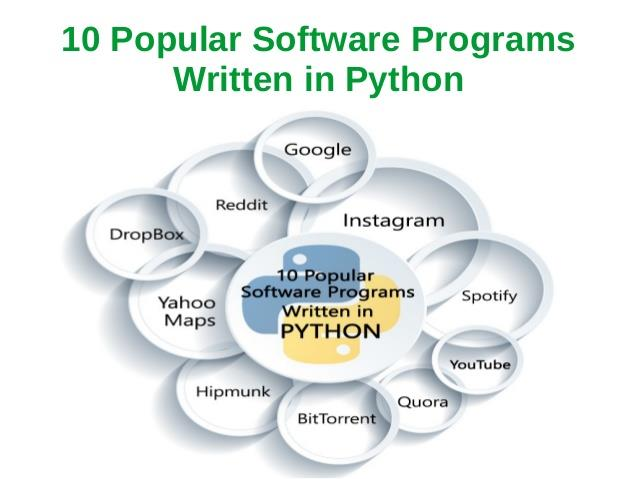
\includegraphics[width=\linewidth/2]{%
    diagrams/programs_written_in_python.png}
  \caption{Popular software written in Python}
\end{figure}
% }}}

% Why we took Python for our project {{{
\subsubsection{Why we took Python for our project}

Python is a well-designed language that can be used for
real world programming. Some of its strengths were very
appealing to us when we thought about which language to
use.

The most obvious strength and the reason we decided to use
Python are the libraries,
frameworks and APIs for machine learning written for/in
Python (especially Tensorflow and Keras, which we used, but
including far more well designed and beloved tools like
PyTorch, Theano, matplotlib, etc).

Here are some other strengths of Python we really
appreciated during development:

\begin{itemize}

  \item System programming:

        Internal interfaces of python that are created for
        working with services of operating system cause
        Python to be a suitable language for system
        programming.

        These interfaces provide some functions such as:
        files and directories operations, parallel
        processing, etc. the standard library of Python can
        support the different types of platforms and
        operating systems. It contains some tools for
        working with system resources such as:
        environmental variables, files, sockets, pipes,
        processes, multiple treats, command line, standard
        stream interfaces, shell programming, etc.
        \cite{amjad21}


  \item Network and internet programming:

        Various modules are embedded in Python standard
        library that provide many tools for network
        programmers, such as: client-server connection,
        socket programming, FTP, Telnet, email functions,
        RPC, SOAP, etc.

        Also, some third-party tools like mod-Python allow
        web servers like apache to run Python scripts.
        Furthermore, some popular programs such as: Django,
        Turbo gears, Pylon, Zope and Web Ware support
        Python scripts.\cite{amjad21}

  \item Numerical programming:

        Python with the NumPy library for Linear Algebra
        computations (used in Tensorflow) can be a powerful
        alternative for FORTRAN and C++, because it
        provides powerful tools for working with
        mathematical libraries, by using simple Python
        code. Also, there are many third-party tools on
        the internet for numerical computations.

\end{itemize}
% }}}


\newpage

\subsection{Neural Networks}\index{Neural Network}

% Derivation from biology {{{
\subsubsection{Derivation from biology}
\label{ss_nn_derivation_from_biology}

"Neural networks are an attempt to model the insights
gained in brain research on the interaction between nerve
cells (neurons) and connections (synapses)".\cite{ct_math}

Here, an artificial neuron\index{Neural Network!artificial
 Neuron} mimics the functioning of a nerve cell. A
biological nerve cell is connected to other nerve cells via
synapses. At these connections, stimuli are transmitted by
means of chemical messengers (neurotransmitters) and
converted into an electrical signal within the nerve cell.

The synapses of a nerve cell are located at so-called
dendrites (branches), from which the transmitted stimuli
are transmitted to the soma (cell body). It does matter how
far the synapse is from the soma. The closer a synapse is
to the soma, the stronger the stimulus transmission.\cite{%
bio,ct_math}

In addition, it should be the case that multiple synapses
stimuli at the same time which adds incoming stimuli within
the nerve cell.\cite{bio} If the stimulus transmitted
exceeds a threshold within the cell, then an action
potential is triggered and the cell forwards the signal to
other cells, which in turn are connected via synapses to
the stimulating transmitting cell. Nerve cells form
associations in the human brain, which develop the ability
to recognize complex structures. Artificial neural networks
are an attempt to imitate these associations of nerve
cells.\cite{ct_math}
% }}}

% Structure of an artificial neuron {{{
\subsubsection{Structure of an artificial neuron}

\begin{figure}[H]
	\begin{center}
	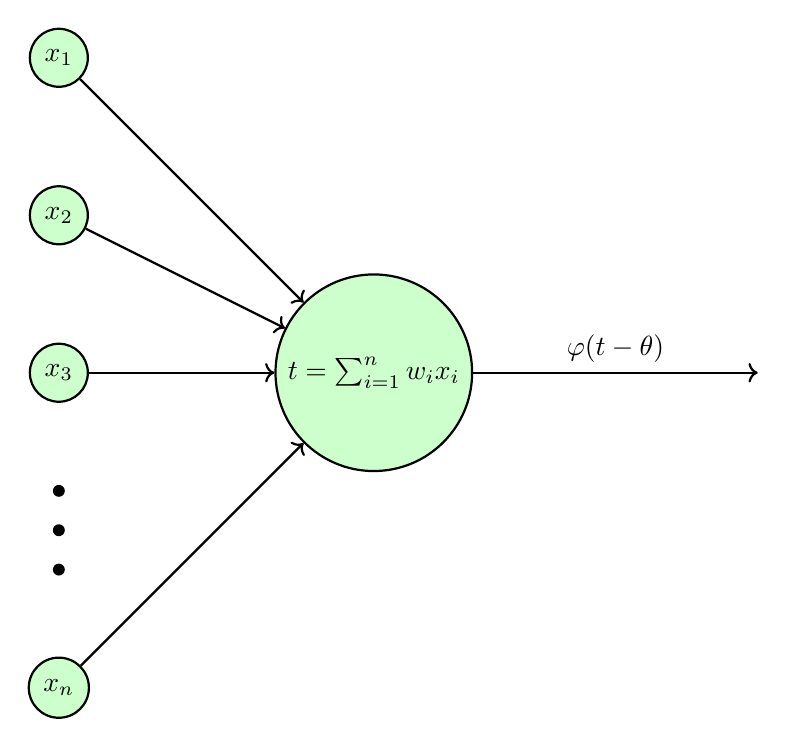
\begin{tikzpicture}[%
    dot/.style={circle,draw,thick,fill=green!20}
  ]
		\node at (5,0) (out) {};
		\node at (0,0) [dot] (neuron) {$t=\sum_{i=1}^{n}{w_ix_i}$}
			edge[->,thick] node[above]{$\varphi(t-\theta)$} (out);
		\node at (-4,4) [dot] {$x_1$}
			edge[->,thick] (neuron);
		\node at (-4,2) [dot] {$x_2$}
			edge[->,thick] (neuron);
		\node at (-4,0) [dot] {$x_3$}
			edge[->,thick] (neuron);
		\node at (-4,-4) [dot] {$x_n$}
			edge[->,thick] (neuron);
		\node at (-4,-1.5) [tokens=1] {};
		\node at (-4,-2) [tokens=1] {};
		\node at (-4,-2.5) [tokens=1] {};
	\end{tikzpicture}
	\end{center}
	\caption{Scheme of an artificial neuron}
	\label{fig_neuron}
\end{figure}



From chapter \ref{ss_nn_derivation_from_biology}, the
components and functioning of an artificial neuron can be
derived.
\newline\newline
In an artificial neuron the following happens:

\begin{enumerate}

  \item An artificial neuron is connected to other neurons
        or the direct value input via input connections,
        which are supposed to represent the synapses of the
        nerve cell (described in Figure \ref{fig_neuron}
        with $x_i$). These inputs can be discreet or
        continuous.\cite{nne_beck}

        If the data comes from other neurons, the weighting
        \index{Neural Network!weighting} of the connection
        is additionally transferred to the value
        $\omega_i$. Each connection of a neuron has an
        individual weighting. The greater the value
        of this weighting, the more important the
        transmitted value $x_i$ for the network output.

  \item The value and weight of each input connection is
        added by the transfer function $\sum_{i=1}^{n}w_ix_i$
        to calculate the net input value $t$.
        \index{Neural Network!net input value}


  \item Every artificial neuron, like a nerve cell, has a
        threshold. An artificial neuron's threshold is a
        value $\theta$\index{Neural Network!threshold}.
        The threshold $\theta$ is subtracted from the net
        input value $t$ to determine the activation
        potential of the neuron.

        The threshold can also be represented by the bias.
        The bias\index{Neural Network!bias} is a further
        input, which transmits the constant value 1 and as
        weighting the value $b=-\theta$.

        	\begin{figure}[H]
		\begin{center}
			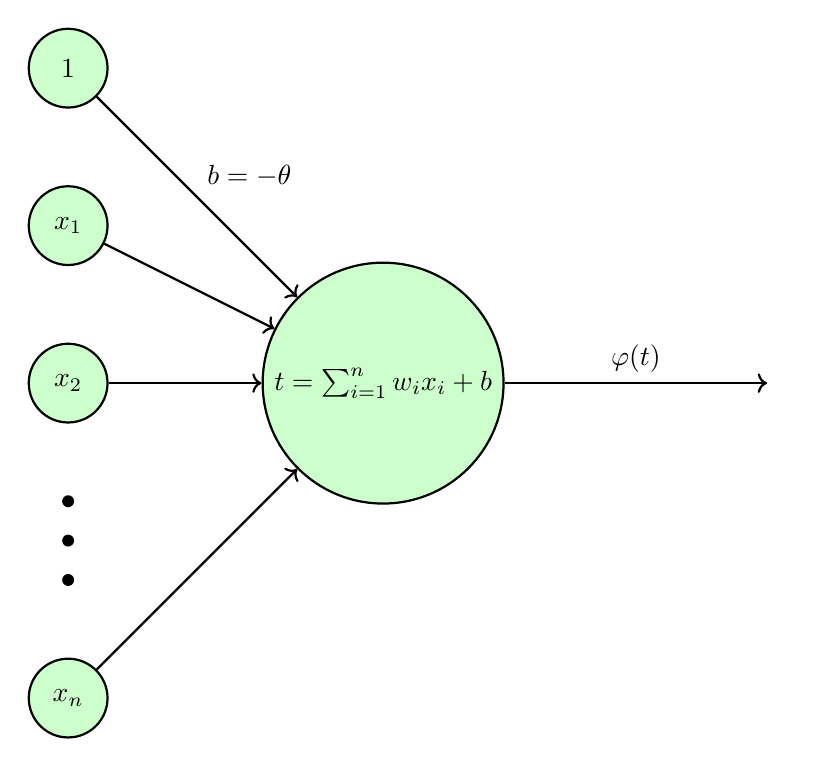
\begin{tikzpicture}[dot/.style={circle,draw,thick,fill=green!20,minimum size=1cm}]
				\node at (5,0) (out) {};
				\node at (0,0) [dot] (neuron) {$t=\sum_{i=1}^{n}{w_ix_i}+b$}
					edge[->,thick] node[above]{$\varphi(t)$} (out);
				\node at (-4,4) [dot] {$1$}
					edge[->,thick] node[anchor=south west]{$b=-\theta$} (neuron);
				\node at (-4,2) [dot] {$x_1$}
					edge[->,thick] (neuron);
				\node at (-4,0) [dot] {$x_2$}
					edge[->,thick] (neuron);
				\node at (-4,-4) [dot] {$x_n$}
					edge[->,thick] (neuron);
				\node at (-4,-1.5) [tokens=1] {};
				\node at (-4,-2) [tokens=1] {};
				\node at (-4,-2.5) [tokens=1] {};
			\end{tikzpicture}
		\end{center}
    \caption{An artificial neuron with bias}
    %\label{bn}
	\end{figure}



  \item The determined value of $t-\theta$ is used as an
        input in the activation function $\varphi$ to
        determine the output of the neuron.
        \index{Neural Network!activation function}

        From this process, the basic elements of a neuron
        can be determined:

        \begin{itemize}

          \item Weighting

          \item Threshold

          \item Transfer function

          \item Activation function

        \end{itemize}

\end{enumerate}
% }}}

% Construction of a neural network {{{
\subsubsection{Construction of a neural network}

\begin{figure}[H]
  \begin{center}
	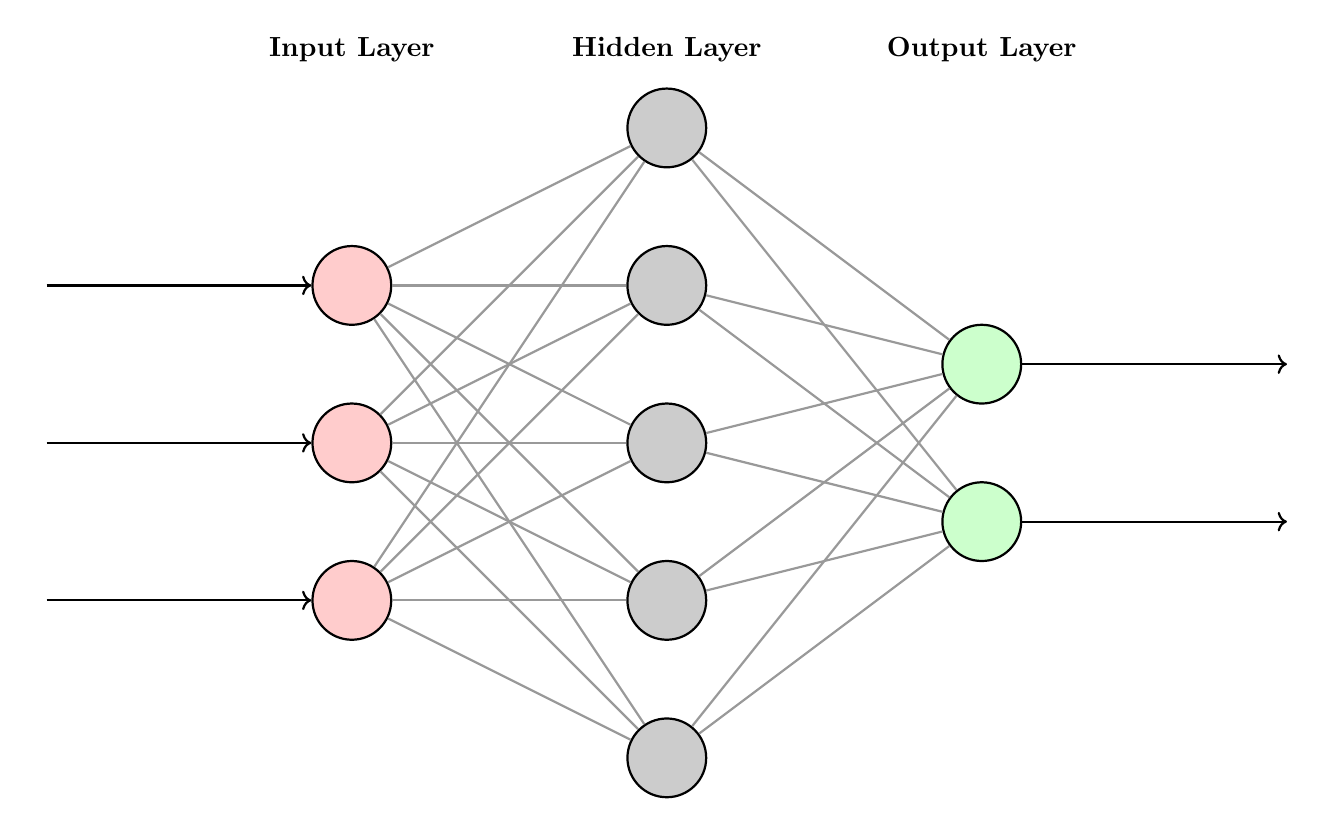
\begin{tikzpicture}[%
    dot/.style={circle,draw,thick,minimum size = 1cm}
  ]
		\node at(-4,5) {\textbf{Input Layer}};
		\node at(0,5) {\textbf{Hidden Layer}};
		\node at(4,5) {\textbf{Output Layer}};

		\node at(8,1) (oo1) {};
		\node at(8,-1) (oo2) {};

		\node at (4,1) [dot,fill=green!20] (o1) {}
			edge[->,thick] (oo1);
		\node at (4,-1) [dot,fill=green!20] (o2) {}
			edge[->,thick] (oo2);

		\node at (0,4) [dot,fill=black!20] (h1) {}
			edge[thick,black!40] (o1)
			edge[thick,black!40] (o2);
		\node at (0,2) [dot,fill=black!20] (h2) {}
			edge[thick,black!40] (o1)
			edge[thick,black!40] (o2);
		\node at (0,0) [dot,fill=black!20] (h3) {}
			edge[thick,black!40] (o1)
			edge[thick,black!40] (o2);
		\node at (0,-2) [dot,fill=black!20] (h4) {}
			edge[thick,black!40] (o1)
			edge[thick,black!40] (o2);
		\node at (0,-4) [dot,fill=black!20] (h5) {}
			edge[thick,black!40] (o1)
			edge[thick,black!40] (o2);

		\node at (-4,2) [dot,fill=red!20] (i1) {}
			edge[thick,black!40] (h1)
			edge[thick,black!40] (h2)
			edge[thick,black!40] (h3)
			edge[thick,black!40] (h4)
			edge[thick,black!40] (h5);
		\node at (-4,0) [dot,fill=red!20] (i2) {}
			edge[thick,black!40] (h1)
			edge[thick,black!40] (h2)
			edge[thick,black!40] (h3)
			edge[thick,black!40] (h4)
			edge[thick,black!40] (h5);
		\node at (-4,-2) [dot,fill=red!20] (i3) {}
			edge[thick,black!40] (h1)
			edge[thick,black!40] (h2)
			edge[thick,black!40] (h3)
			edge[thick,black!40] (h4)
			edge[thick,black!40] (h5);

		\node at(-8,2) (ii1) {}
			edge[->,thick] (i1);
		\node at(-8,0) (ii2) {}
			edge[->,thick] (i2);
		\node at(-8,-2) (ii3) {}
			edge[->,thick] (i3);
	\end{tikzpicture}
  \end{center}
  \caption{Neural network with hidden layer}
  %\label{snn}
\end{figure}


Neural networks are built in several levels (layers). Each
of these layers consists of a certain number of neurons and
connections. Each neuron of a layer is connected to all
neurons of the next layer via the already discussed
weighted input connections.

\begin{itemize}

  \item \textbf{Input layer:}

        The input layer is the first layer of a neural
        network. It contains the same Number of neurons,
        such as input and output values in the test and
        learning data available.
        \index{Neural Network!Layers!Input Layer}

  \item \textbf{Hidden layer:}

        A neural network can not contain, one or more
        hidden layers. Neural networks can solve simple
        problems without hidden layers, many problems, such
        as the so-called "XOR problem", can't be solved
        without at least one of these layers.\cite{nne_beck}

        The hidden layers consist of neurons, which
        together represent an internal representation of
        the input. The weighting to the individual neurons
        of the hidden layer is determined, for example, by
        means of back propagation.
        \index{Neural Network!Layers!Hidden Layer}

  \item \textbf{Output Layer:}

        The output layer is the last layer of a neural
        network. It delivers the results of the network to
        the outside world. The number of neurons in the
        output layer equals the number of expected output
        values.
        \index{Neural Network!Layers!Output Layer}


\end{itemize}
% }}}

% Learning algorithms {{{
\subsubsection{Learning algorithms}

Each neural network must be trained with training records.
These records consist of rows with the input values and the
expected output (supervised learning). The training itself
is an iterative process in which each input and output
passes through rows.\cite{ct_math}

In order for the network to learn how to approximate the
output value, the weights and threshold of each neuron must
be modified and adjusted.

The quality measure is the quadratic cost function:

\begin{align*}
  E = \frac{1}{2}\sum_{i=1}^{n}(a_i-o_i)^2
\end{align*}

The network error $E$ consists of the accumulated squared
deviations of the individual rows.

These are calculated from the difference between the
expected output value $a_i$ and the calculated network
output $o_i$. The sum is multiplied by $\frac{1}{2}$. This
factor simplifies the derivation. The aim now is to find
the combination of thresholds and weights of the neurons in
which the network error $E$ is the lowest.

You could now let the net simply try all possible weights
and thresholds until the combination with the smallest
error $E$ is found. This is not possible in practice, as
there are usually too many parameters that have to be tried
out within the network.\cite{ct_math}

For this purpose, learning algorithms are used instead.
Learning algorithms distinguish between two categories,
supervised and unsupervised learning.
% }}}

% Reinforcement learning {{{
\subsubsection{Reinforcement Learning}

Reinforcement learning (RL) is an area of machine learning,
inspired by behaviorist psychology, concerned with how
software agents ought to take actions in an environment so
as to maximize some notion of cumulative reward.
\index{Reinforcement Learning}

The problem, due to its generality, is studied in many
other disciplines, such as game theory, control theory,
operations research, information theory, simulation-based
optimization, multi-agent systems, swarm intelligence,
statistics and genetic algorithms. In the operations
research and control literature, reinforcement learning is
called approximate dynamic programming, or neuro-dynamic
programming.

The problems of interest in reinforcement learning have
also been studied in the theory of optimal control, which
is concerned mostly with the existence and characterization
of optimal solutions, and algorithms for their exact
computation, and less with learning or approximation,
particularly in the absence of a mathematical model of the
environment. In economics and game theory, reinforcement
learning may be used to explain how equilibrium may arise
under bounded rationality.\cite{wrl}

While neural networks are responsible for recent
breakthroughs in problems like computer vision, machine
translation and time series prediction – they can also
combine with reinforcement learning algorithms to create
something astounding like AlphaGo.\cite{alphago}

Reinforcement learning refers to goal-oriented algorithms,
which learn how to attain a complex objective (goal) or
maximize along a particular dimension over many steps; for
example, maximize the points won in a game over many moves.
They can start from a blank slate, and under the right
conditions they achieve superhuman performance. Like a
child incentivized by spankings and candy, these algorithms
are penalized when they make the wrong decisions and
rewarded when they make the right ones – this is
reinforcement. Reinforcement algorithms that incorporate
deep learning can beat world champions at the game of Go as
well as human experts playing numerous Atari video games.
While that may sound trivial, it’s a vast improvement over
their previous accomplishments, and the state of the art is
progressing rapidly.\cite{alphago}

Reinforcement learning solves the difficult problem of
correlating immediate actions with the delayed returns they
produce. Like humans, reinforcement learning algorithms
sometimes have to wait a while to see the fruit of their
decisions. They operate in a delayed return environment,
where it can be difficult to understand which action leads
to which outcome over many time steps.

Reinforcement learning algorithms can be expected to
perform better and better in more ambiguous, real-life
environments while choosing from an arbitrary number of
possible actions, rather than from the limited options of a
video game. That is, with time we expect them to be
valuable to achieve goals in the real world.\cite{aiw}
% }}}

% Neural Networks and Deep Reinforcement Learning {{{
\subsubsection{Neural Networks and Deep Reinforcement
  Learning}
\label{ss_nn_nndrl}

Where do neural networks fit in with RL? Neural networks
are the agent that learns to map state-action pairs to
rewards. Like all neural networks, they use coefficients to
approximate the function relating inputs to outputs, and
their learning consists to finding the right coefficients,
or weights, by iteratively adjusting those weights along
gradients that promise less error.
\index{Reinforcement Learning!agent}
\index{Reinforcement Learning!reward}
\index{Reinforcement Learning!action}
\index{Reinforcement Learning!state (observation)}

In reinforcement learning, convolutional networks can be
used to recognize an agent's state; e.g.\ the screen that
Mario is on, or the terrain before a drone. That is, they
perform their typical task of image recognition.

But convolutional networks derive different interpretations
from images in reinforcement learning than in supervised
learning. In supervised learning, the network applies a
label to an image; that is, it matches names to pixels.

In reinforcement learning, given an image that represents a
state, a convolutional net can rank the actions possible to
perform in that state; for example, it might predict that
running right will return 5 points, jumping 7, and running
left none.

\begin{figure}[H]
  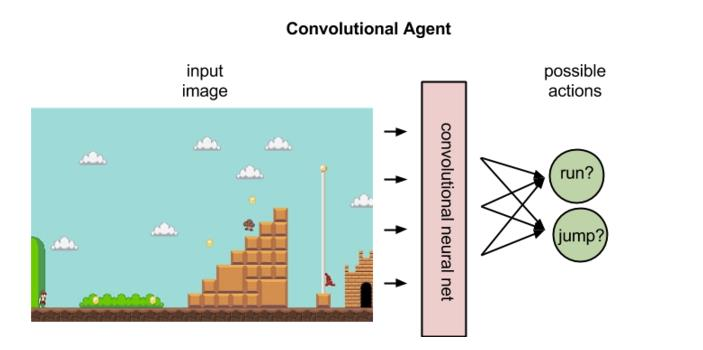
\includegraphics[width=\linewidth]{%
    diagrams/convolution_agent.PNG}
  \caption{Convolutional Agent\cite{aiw}}
\end{figure}

The above image illustrates what a policy agent does,
mapping a state to the best action.


At the beginning of reinforcement learning, the neural
network coefficients may be initialized stochastically, or
randomly. Using feedback from the environment, the neural
net can use the difference between its expected reward and
the ground-truth reward to adjust its weights and improve
its interpretation of state-action pairs.

Reinforcement learning relies on the environment to send it
a scalar number in response to each new action. The rewards
returned by the environment can be varied, delayed or
affected by unknown variables, introducing noise to the
feedback loop.\cite{aiw}

\begin{figure}[H]
  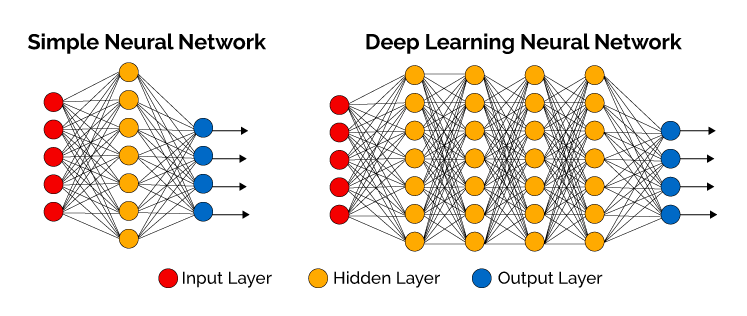
\includegraphics[width=\linewidth]{%
    diagrams/deep_learning.png}
  \caption{Difference between a Deep Learning Network and
    a Neural Network}
\end{figure}

The typical framing of a Reinforcement Learning (RL)
scenario: an agent takes actions in an environment, which
is interpreted into a reward and a representation of the
state, which are fed back into the agent.

\begin{figure}[H]
  \centering
  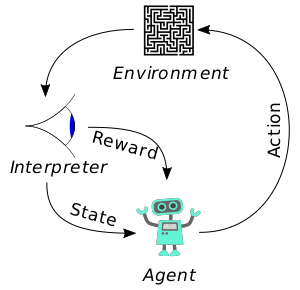
\includegraphics[width=\linewidth/2]{%
    diagrams/reinforcement_learning.png}
  \caption{Reinforcement learning diagram\cite{wrl}}
\end{figure}
% }}}


\newpage

\subsection{OpenAI Gym}
\label{s_openai_gym}

"OpenAI Gym is a toolkit for reinforcement learning
research. It includes a growing collection of benchmark
problems that expose a common interface, and a website
where people can share their results and compare the
performance of algorithms."\cite{gym}
\index{OpenAI Gym}

OpenAI Gym is an easy to use and easy to integrate toolkit
with a veriety of environments for reinforcement learning
(RL) (cmp. \ref{ss_nn_nndrl}) which we used for training
our agent. An environment can be a retro arcade game (used
in our project) or some other complex task which the agent
should master.
\index{OpenAI Gym!environments}

\begin{figure}[H]
\begin{mdframed}[style=codebox]
\begin{lstlisting}[language=Python]
# a small example program using OpenAI Gym

import gym
import random

# build gym environment. A full list of available environ-
# ments can be found at: https://gym.openai.com/envs/
environment = gym.make('LunarLander-v2')

# the range of actions an agent can perform. As a mathemat-
# ical set: [0..action_space[
action_space = environment.action_space.n

# mandatory first reset
environment.reset()

# generate random action (instead of predicted action from
# the agent)
action = random.randrange(0,action_space)

# observations provided by the gym environment after
# doing the random action in the environment.
observation, reward, done, info = environment.step(action)

\end{lstlisting}
\end{mdframed}
\caption{A small example program using OpenAI Gym}
\end{figure}

Important for further understanding of how we utilized gym
is the concept of episodes. An episode is a finite sequence
of actions performed on the environment which either
concludes in solving the environment (reaching a specific
score which is different for each environment) or failing,
basically representing a game played.
\index{OpenAI Gym!episodes}

\begin{figure}[H]
\begin{mdframed}[style=codebox]
\begin{lstlisting}[language=Python]
# example of an episode

# if the episode reaches this score the episode is finished
# successfully
score_solved = 200

# the score reached in this episode
score = 0

# perform the finite sequence of actions (terminated by
# the environment)
while True:

  # generate random action (instead of predicted action
  # from the agent)
  action = random.randrange(0,action_space)

  # observations provided by the gym environment after
  # doing the random action in the environment
  observation, reward, done, info = environment.step(action)

  # add the reward from the action to the overall reached
  # score of the episode
  score += reward

  # the done value provided by the environment is a Boolean
  # which specifies if the episode is finished (either suc-
  # cessfully or not)
  if done:
    if score == score_solved:
      print("finished episode successfully!")
    else:
      print("failed episode!")

    # reset environment after every episode (otherwise gym
    # throws an exception when calling env.step, since the
    # episode already terminated)
    env.reset()

    # return from episode loop
    break
\end{lstlisting}
\end{mdframed}
\caption{Example of an episode (game) played on an OpenAI
  Gym environment}
\end{figure}

An agent has solved an environment if it succeeded $x$
consecutive episodes. $x$ is provided by Gym.


\newpage

\subsection{Tensorflow}

\newpage

\subsection{Message Broker}
\label{s_message_broker}

% Introduction {{{
A message broker is an intermediary computer program module
that translates a message from the formal messaging
protocol of the sender to the formal messaging protocol of
the receiver.

Message brokers are elements in telecommunication or
computer networks where software applications communicate
by exchanging formally-defined messages. Message brokers
are a building block of message-oriented middleware (MOM)
but are typically not a replacement for traditional
middleware like MOM and remote procedure call (RPC).
\cite{amjad27}
% }}}

% History {{{
\subsubsection{History}

Message broker products are the middleware that embody
different messaging solutions. In 1983 Vivek Ranadivé from
Teknekron Software Systems began working on an idea based
on the ideals of a Software Bus to enable applications to
share data in a standard fashion. That work would later be
referred to as “The Information Bus”. Already in 1986 his
ideas were put to use when Goldman Sachs, an American
investment banking firm, launched cooperation with
Teknekron to find solutions for the trading floor of the
future.\cite{amjad28}

For nearly two decades the domain of message exchange was
left for proprietary vendors and proprietary formats.
Throughout the 1980s and 1990s message queuing kept
evolving but in isolation since commercial message queue
vendors strived for interoperability between client
applications rather than worked on standardized interfaces
for their message queuing products to utilize.
\cite{amjad28}


The figure bellow shows a brief timeline of message queuing:

\begin{figure}[H]
  \centering
  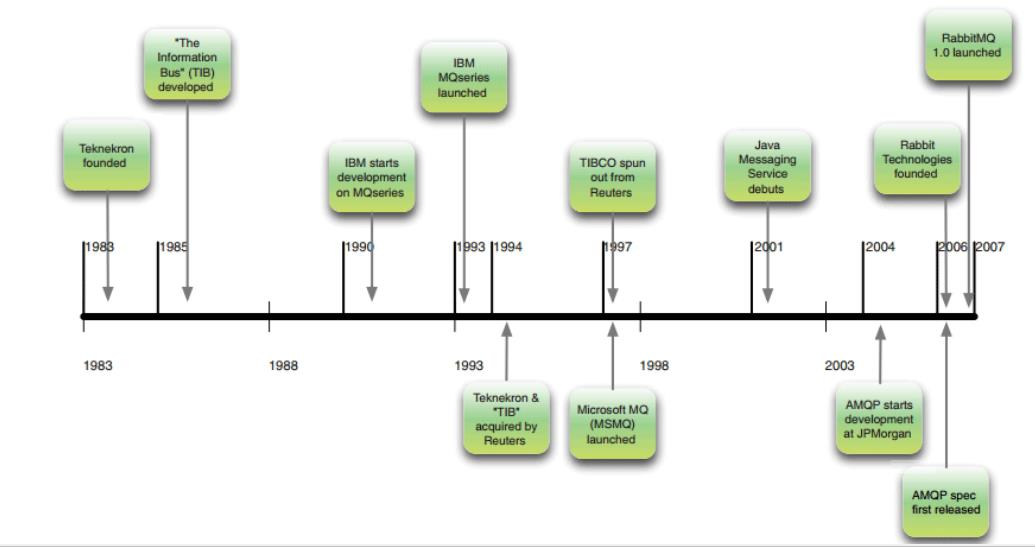
\includegraphics[width=\linewidth]{%
    diagrams/messaging_history.png}
  \caption{Timeline of message queuing}
\end{figure}
% }}}

% Functionality and architecture {{{
\subsubsection{Functionality and architecture}
\label{ss_mb_faa}

A message broker is an architectural pattern for message
validation, transformation, and routing.

It mediates communication among applications, minimizing
the mutual awareness that applications should have of each
other in order to be able to exchange messages, effectively
implementing decoupling.\cite{amjad29}

The primary purpose of a broker is to take incoming
messages from applications and perform some action on them.
Message brokers can decouple endpoints, meet specific non-
functional requirements, and facilitate reuse of
intermediary functions. For example, a message broker may
be used to manage a workload queue or message queue for
multiple receivers, providing reliable storage, guaranteed
message delivery and perhaps transaction management.
\cite{amjad27}

Message brokers are generally based on one of two
fundamental architectures: hub-and-spoke and message bus.
In the prior, a central server acts as the mechanism that
provides integration services, whereas with the latter, the
message broker is a communication backbone or distributed
service that acts on the bus.\cite{amjad30}

\begin{figure}[H]
  \centering
  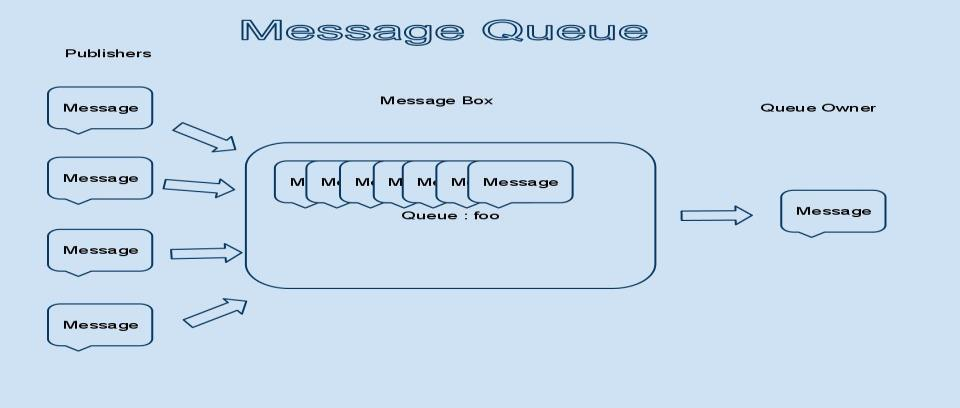
\includegraphics[width=\linewidth]{%
    diagrams/message_queue.png}
  \caption{Scheme of a message queue}
\end{figure}
% }}}

\subsection{RabbitMQ}
\label{s_rabbitmq}
\index{RabbitMQ}

% Introduction {{{
\begin{figure}[H]
  \centering
  
\includegraphics[width=\linewidth/2]{%
    diagrams/rabbitmq_logo.png}
  \caption{RabbitMQ Logo}
\end{figure}

For our project we used RabbitMQ as our messsage broker.

RabbitMQ is an open source message broker software
(sometimes called message-oriented middleware) that
originally implemented the Advanced Message Queuing
Protocol(AMQP) and has since been extended with a plug-in
architecture to support Streaming Text Oriented Messaging
Protocol (STOMP), Message Queuing Telemetry Transport
(MQTT), and other protocols.\cite{amjad22}

The RabbitMQ server program is written in the Erlang
programming language and is built on the Open Telecom
Platform framework for clustering and failover. Client
libraries to interact with the broker are available for all
major programming languages.\cite{amjad23}
% }}}

% Small glance on the history of RabbitMQ {{{
\subsubsection{Small glance on the history of RabbitMQ}

Rabbit Technologies Ltd., originally developed RabbitMQ.
Rabbit Technologies started as a joint venture between
LShift and CohesiveFT in 2007\cite{amjad24}, and was
acquired in April 2010 by SpringSource, a division of
VMware.\cite{amjad25} The project became part of Pivotal
Software in May 2013.\cite{amjad26}

% }}}


\section{Application}

% Introduction {{{
Our goal was to make use of a lot of computing power in
order to train our agent to master an OpenAI Gym
Environment (cmp. \ref{s_openai_gym}). In this chapter we
will document how we tried to achieve this goal with our
distributed application.
\index{Application}

% }}}

% The agent {{{
\subsection{The agent}
\label{s_agent}

Before going into detail on the application's architecture,
here is a brief summary on what our agent actually is.

We programmed our agent as a neural network with the Keras
library, which has an API for high level, high abstraction
neural networks.

Keras uses Tensorflow as its backend for computations and
basically only provides a nicer abstraction of Tensorflow.

% example {{{
\begin{mdframed}[style=codebox]
\begin{lstlisting}[language=Python]
# a small example program using Keras
#
# API documentation at: https://keras.io/

# Sequential is the keras object representing a neural net-
# work
from keras.models import Sequential
# a neural net is comprised of layers connected with each
# other. The Dense object represents a layer
from keras.layers import Dense

# the neural net. This specific neural net has four layers
# (the input (size of 12), two hidden (both 64 artificial
# neurons) and the output layer (size of 4)). The input
# layer does not have to be specified since the input_dim
# parameter of the first layer automatically generates the
# input layer.
model = Sequential([
  Dense(64, activation='relu', input_dim=12 ),
  Dense(64, activation='relu'               ),
  Dense(4,  activation='softmax'            ),
])

# define how the model should learn and some other meta
# information for the training process (learning algorithm,
# optimizer, etc)
model.compile(
        optimizer = 'adam',
        loss      = 'categorical_crossentropy',
        metrics   = ['accuracy']
)

# generate a dummy data set with corresponding labels with
# 1000 entries for training
import numpy as np

data   = np.random.random((1000,12))
# generating the labels (either a 0 or a 1)
labels = np.random.randint(2, size=(1000, 1))

# training the model, iterating 10 times
model.train(data, labels, epochs=10)

# using the neural net to predict the label of a random
# data point
test   = np.random.random((1,12))

model.predict(test)
\end{lstlisting}
\end{mdframed}
\begin{figure}[H]
\caption{A small example program using Keras}
\end{figure}
% }}}

Our agent has the observation provided by the Gym
environment (cmp. \ref{s_openai_gym}) as its input
parameters and as output parameters the actions (the size
of the output layer equals the action space $a$
($|[0..a[| = a$) of the Gym environment.

% }}}


\newpage

\subsection{Architecture}

This chapter will describe in detail how our application
is build, how it works and what we use to achieve
concurrency.

On a higher level our application is devided into two
distinct parts, the Executor ($E$) and the Worker ($W$).

$E$ is the part of our application that is doing the
training and testing of our agent, while  $W$ generates
training data which is sent via the RabbitMQ to $E$ so $E$
can train the agent with this data. After training $E$
sends the agent to $W$ so $W$ can generate new training
data with the updated agent.

This iteration is continued until the agent is able to
solve the Gym environment (cmp. \ref{s_openai_gym}).

% Network {{{
\subsubsection{Network}

Instances of both, $E_i$ and $W_j$ communicate over a
message broker, in this case RabbitMQ (cmp.
\ref{s_message_broker}, \ref{s_rabbitmq}).

\input{diagrams/app_network}
% }}}


\subsubsection{Executor}
\label{s_executor}
\index{Application!Executor}

The Executor $E$ is the part of the application that is
doing the training and testing of our agent. Training and
testing is done incrementally in a loop, the "TTSL"
(Training-Testing-Sending-Loop). An Executor instance
$E_i$ gets provided with its training data from the Worker
instances $W_j$ it is connected to (via the RabbitMQ).

If the testing part of the "TTSL" failed $E_i$ sends the
newly trained agent to every $W_j$ (the sending part of the
"TTSL"). Else if the testing was successful and the agent
mastered the environment (cmp \ref{s_openai_gym}) it sends
a message that testing was successful which kills every
$W_j$.

The Executor is composed of three processes, the main
process, the meta process and the TTSL process.

\begin{itemize}[label={}]

  \item \textbf{main process:}

        The main process first initializes global shared
        variables and constants it shares with the other
        two processes. Then it starts the meta process and
        the TTSL process.

        After that the main process becomes a listener
        which listens for incoming data from the Worker
        instances connected to the RabbitMQ. If new data
        comes in it is saved in a shared variable so the
        TTSL process can access it.
        \index{Application!Executor!main process}

  \item \textbf{TTSL process:}

        The process executing the TTSL.
        \index{Application!Executor!TTSL process}

  \item \textbf{meta process:}

        This process is a listener (like main becomes after
        initializing the shared memory and starting this
        and the TTSL process) which listens to a queue
        of the RabbitMQ so this Executor can communicate
        with the Workers it is connected to.
        \index{Application!Executor!meta process}

\end{itemize}

\input{diagrams/executor_process}


\subsubsection{Worker}
\label{s_worker}
\index{Application!Worker}

The Worker $W$ is the part of the application that is
generating the data set for training the agent. The
generation of the training data set is the most expensive
task when it comes to computational effort.

While doing the generation $W$ is playing $x$ many episodes
consecutively. $x$ is statically provided by us and is
known at runtime. After finishing an episode the the score
of this episode is decisive wether the episode is good
enough for the training set, since the quality of the
training data set is very crucial for the agent to succeed.

Quality management is done statically with some constants
(like $x$).

Since generating training data is so expensive and can be
done concurrently we use many processes controlled by a
Python object called ProcessPoolExecutor from the
concurrent.futures part of Python's standard library for
this task.
\index{ProcessPoolExecutor}

\begin{figure}[H]
\begin{mdframed}[style=codebox]
\begin{lstlisting}[language=Python]
# a small example program using a ProcessPoolExecutor
from concurrent import futures

# this is executed by every process. Every process gets
# an id (i) which is used as a factor for computing a power
# sequence in the range(100*i,100*i+100)
def power_sequence(i):
  start  = 100*i
  end    = start + 100
  _powers = []

  for i in range(start, end):
    _powers += i**i

  return _powers

# the list of powers
powers = []

# the ProcessPoolExecutor that starts 10 processes which
# means a power sequence for range 0..999 is generated
with futures.ProcessPoolExecutor(max_workers=10) as e:
  # safe every process in fs
  fs = [e.submit(power_sequence,i) for i in range(10)]

  # await the return
  for f in futures.as_completed(fs):
    powers += f.result()

print(powers)
\end{lstlisting}
\end{mdframed}
\caption{A small example program using ProcessPoolExecutor}
\end{figure}

Concurrent, multiprocessing and thread are the parts of
Python's standard library wich provide rich features for
concurrent programming.

While concurrent provides higher-level abstractions which
are more easy to use, multithreading provides the more
low-level, more powerful APIs for concurrent programming
such as a standalone Process object, Locks (mutexes),
Semaphores, Pipes, Queues or ProxyObjects
(shared variables).

We use multiprocessing for spawning standalone processes,
sharing variables and for mutexes (synchronization between
processes).

Like the Executor (cmp. \ref{s_executor}) a Worker instance
is composed of more than one process. But while an
Executor needs three, a Worker needs only two processes.

\begin{itemize}[label={}]

  \item \textbf{main process:}

        Like the Executor the Worker first initializes
        some static or shared variables and constants.
        But after the initialization part the worker has
        to get some information first before continuing
        execution.

        Since the Worker should be able to run like a
        daemon waiting for his task (provided by an
        Executor) the Worker needs the information which
        environment he should generate test data for.

        This information is provided by an Executor
        instance connected to the RabbitMQ. The Worker
        sends periodically a message to a queue the
        Executors meta process listens to. The Executor
        instance than answers with the name of the
        environment the Worker should use. The environment
        is specified by us when starting the Executor via
        its CLI.

        While it is possible to connect many Executors to
        the RabbitMQ, they all can only be started with
        the same environment since otherwise corrupt data
        will destroy any chance of success (we did not
        implement a way to distinguish between different
        environments using the same RabbitMQ).

        After having the environment the main process can
        continue.

        The main process then starts the Worker's
        generating unit called "GSL" (Generate-Send-Loop).
        This is the loop corresponding to the Executors
        "TTSL" unit.

        Followed by that the main process becomes a
        listener for a queue on the RabbitMQ. On that queue
        the main process gets the new agent provided by an
        Executor instance which is shared with the GSL
        process or a message which says that the agent
        succeeded. If that is the case the main process
        answers with a protocol to the queue the meta
        process of the Executor listens to and then kills
        the GSL process and itself.
        \index{Application!Worker!main process}

  \item \textbf{GSL process:}

        The GSL generates and sanitizes the test data
        before sending it to the Executor. For that it uses
        Python's above mentioned ProcessPoolExecutor.

        Since the Worker is not provided with an agent yet
        it generates the actions performed in every episode
        played randomly.

        After the first batch of training data the Executor
        has processed, the Executor can send the first
        version of its agent to the Worker which can use it
        for generation afterwards.

        It should be noted that the Worker not only uses
        the agent for generating new training data but also
        spawns some processes which generate training data
        randomly so the agent does not start to make the
        same mistakes over and over again.
        \index{Application!Worker!GSL process}

\end{itemize}

\input{diagrams/worker_process.tex}


\subsubsection{Queues and Exchanges}

Now, this chapter will go more into detail on how we
utilize the RabbitMQ.

First, there are two concepts we used for communication
with the RabbitMQ called queues and exchanges.

\begin{itemize}[label={}]

  \item \textbf{queue:}

        This concept we already discussed in chapter
        \ref{ss_mb_faa}. Now, for our project one property
        of a queue is interesting, which is "first come,
        first serve" or "FIFO" (First In, First Out), which
        means once a message is received by a listener
        (also called consumer), other listeners (consumers)
        that subscribed to this particular queue will never
        receive this message and all subscribed listeners
        are in a race condition for the next message.

        Because of this we need another concept for
        distributing certain messages (e.g. sending our
        agent to each Worker, since every Worker should use
        a current version of the agent wich would not be
        possible if a Executor would send the agent to a
        queue, because then only one would receive the new
        agent instead of all Workers).

  \item \textbf{exchange:}

        For the above mentioned szenario we need a
        different message distribution called
        publish/subscribe.

        Publish/subscribe message distribution can be
        achieved with an exchange provided by the RabbitMQ.

        In this szenario the Executor would by the
        publisher while the Workers would be the
        subscribers. For every listener (subscriber)
        RabbitMQ generates a new queue and redistributes
        every message published to the exchange to the
        queues.

        For this redistribution or routing are some methods
        available. We only used the method called fanout,
        which generates a copy of every published message
        for each listener (consumer) receiving on an
        exchange.

\end{itemize}

\begin{figure}[H]
\begin{center}
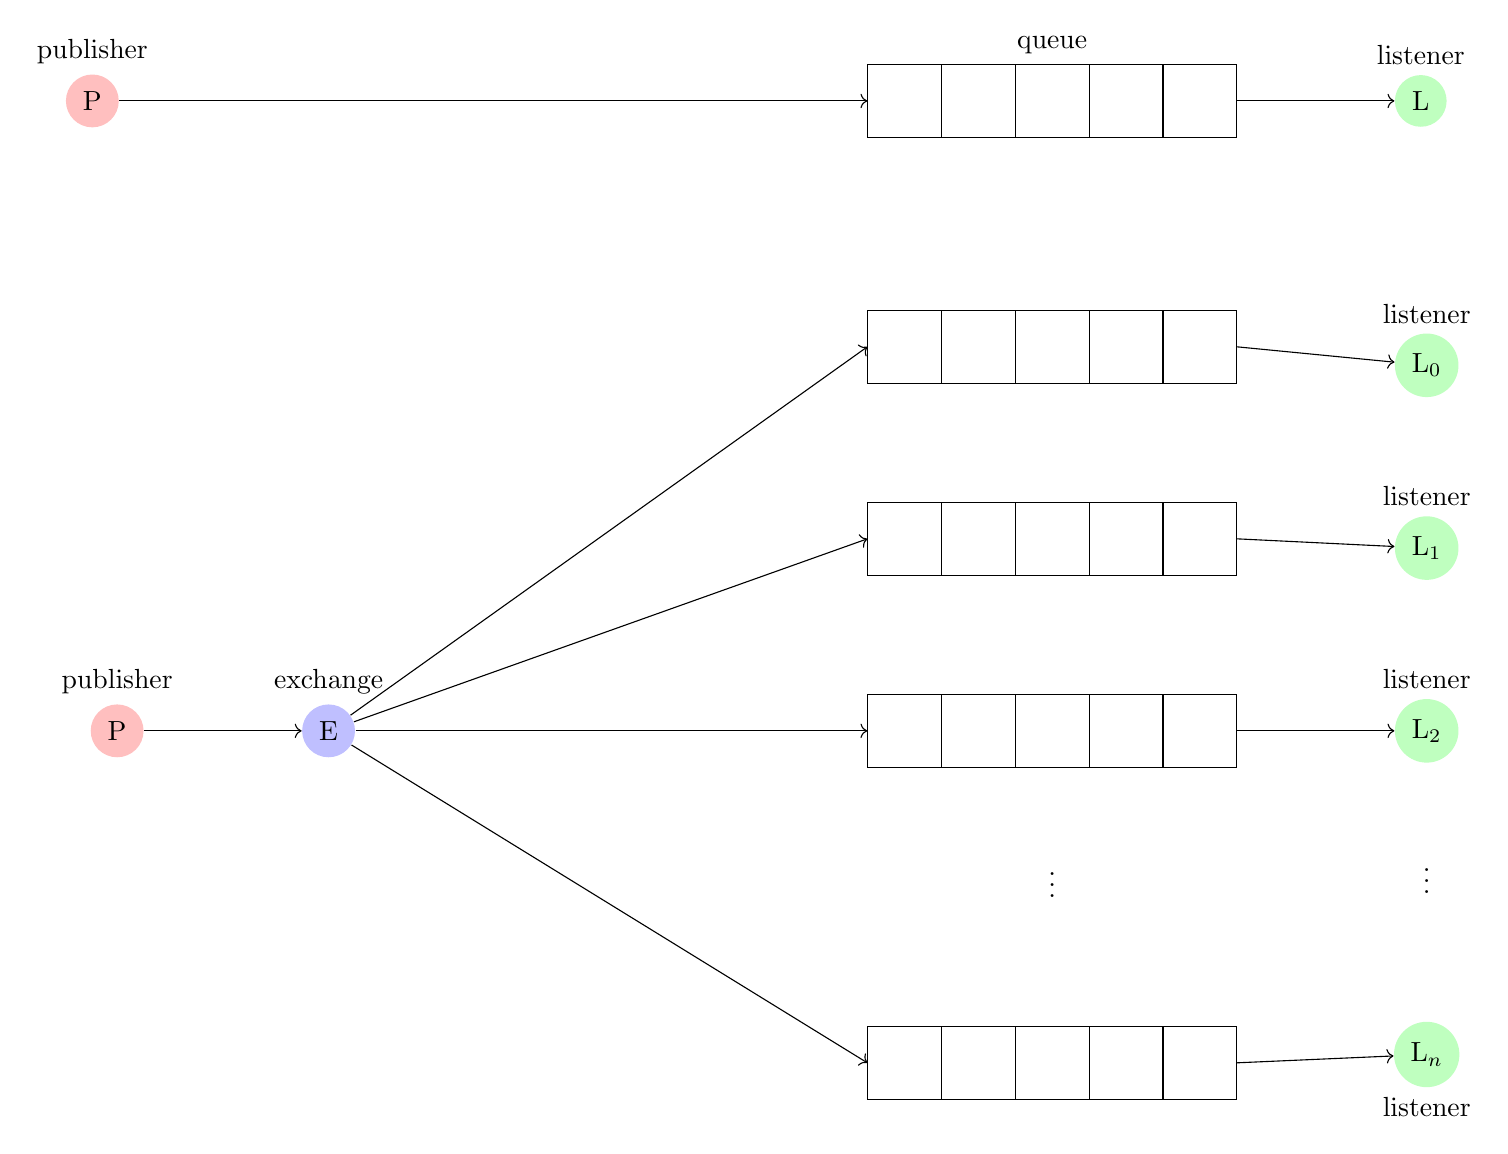
\begin{tikzpicture}

\node[rectangle split, rectangle split parts = 5,
      rectangle split ignore empty parts=false,
      rectangle split horizontal,
      inner sep=11pt, draw, label=queue]
  at (0,0) (queue) {};

\node[circle,fill=red!25,left=9.5 of queue,label=publisher]
  {P}
  edge[->] (queue);

\node[circle,fill=green!25,right=2 of queue,label=listener]
  {L}
  edge[<-] (queue);



\node[rectangle split, rectangle split parts = 5,
      rectangle split ignore empty parts=false,
      rectangle split horizontal,
      inner sep=11pt, draw]
  at (0,-8) (queue_two) {};

\node[rectangle split, rectangle split parts = 5,
      rectangle split ignore empty parts=false,
      rectangle split horizontal,
      inner sep=11pt, draw, above=1.5 of queue_two]
  (queue_one) {};

\node[rectangle split, rectangle split parts = 5,
      rectangle split ignore empty parts=false,
      rectangle split horizontal,
      inner sep=11pt, draw, above=1.5 of queue_one]
  (queue_zero) {};

\node[below=1 of queue_two] (queue_dots) {\vdots};

\node[rectangle split, rectangle split parts = 5,
      rectangle split ignore empty parts=false,
      rectangle split horizontal,
      inner sep=11pt, draw, below=1.5 of queue_dots]
  (queue_n) {};


\node[circle,fill=blue!25,left=6.5 of queue_two,
      label=exchange]
  (exchange) {E}
  edge[->] (queue_two.west)
  edge[->] (queue_one.west)
  edge[->] (queue_zero.west)
  edge[->] (queue_n.west);


\node[circle,fill=red!25,left=2 of exchange,
      label=publisher]
  {P}
  edge[->] (exchange);


\node[circle,fill=green!25,right=2 of queue_two,
      label=listener]
  (l_two) {L$_2$}
  edge[<-] (queue_two.east);

\node[circle,fill=green!25,label=listener,
      above=1.5 of l_two]
  (l_one) {L$_1$}
  edge[<-] (queue_one.east);

\node[circle,fill=green!25,right=2 of queue,label=listener,
      above=1.5 of l_one]
  {L$_0$}
  edge[<-] (queue_zero.east);

\node[below=1 of l_two] (l_dots) {\vdots};

\node[circle,fill=green!25,right=2 of queue,
      label={below:listener},
      below=1.5 of l_dots]
  {L$_n$}
  edge[<-] (queue_n.east);

\end{tikzpicture}
\end{center}
\caption{Scheme of a queue and an exchange}
\end{figure}


The queues and exchanges we used in our project:

\begin{itemize}[label={}]

  \item \textbf{meta\_queue:}

        Queue the meta process of the Executor(s) is/are
        listening to. This queue is used by Workers to
        ask for the environment and for sending the
        protocol once the agent succeeded.

  \item \textbf{meta\_exchange:}

        Corresponds to meta\_queue. The Executor(s) is/are
        answering with the environment on this exchange.

  \item \textbf{data\_queue:}

        Queue used by the Workers to send their generated
        training data to the Executor(s).

  \item \textbf{model\_exchange:}

        Exchange the Executor(s) use(s) for sending the new
        agent to each Worker or, if the agent succeeded,
        for sending a message telling each Worker to send
        their protocols and shut down afterwards.

\end{itemize}



\subsection{Results}

First, we started developing our application for a Gym
(cmp. \ref{s_openai_gym}) environment called "CardPole-v1".
\index{OpenAI Gym!environments!CardPole-v1}

In this environment the agent learns how to balance a stick
moving a board on wich this stick stands either right or
left.

\begin{figure}[H]
  \centering
  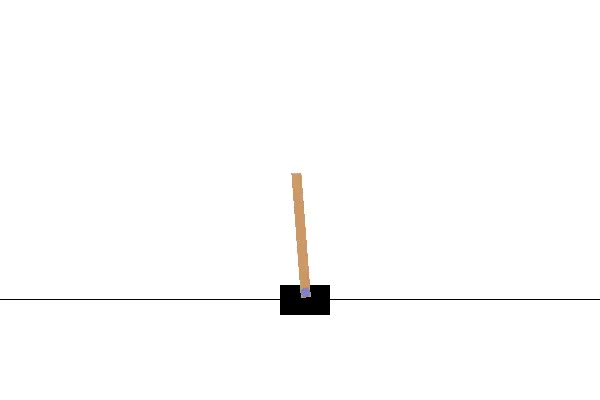
\includegraphics[width=\textwidth/2]
  {diagrams/cardpole.jpg}
  \caption{Screenshot of "CardPole-v1"}
\end{figure}

We developed our program on a HP EliteBook 8730w with a
Intel Core 2 Duo processor (2.40 GHz) running OpenSuSE
Leap 43. We needed an older Tensorflow version because the
current version does not support this CPU anymore. Also
Tensorflow was not able to utilize any GPU (Graphical
Processing Unit), which means our development environment
does not have much computing power to offer.
\index{Application!development environment}

The problem we faced with training an agent for
"CardPole-v1" was that, running the program in our
development environment, we were able to build an agent
that succeded this environment in at most three training
loops (which overall took aproximately 5 minutes). This was
achieved with running one Executor, the RabbitMQ and
between one and three Worker instances on the same device
which does not offer great computing abilitites (especially
compared to the operational environment (the cluster in
Room 1.242 containing 10 Apple Mac Pros)).
\index{Application!operational environment}

Since it would not made much sense running benchmarks on
the operational environment training an agent to master
"CardPole-v1" we needed a different Gym environment.

We decided we would take "LunarLander-v2", a Atari Arcade
Game where the agent has to land an ufo safely inside a
flagged area on the ground.
\index{OpenAI Gym!environments!LunarLander-v2}

\begin{figure}[H]
  \centering
  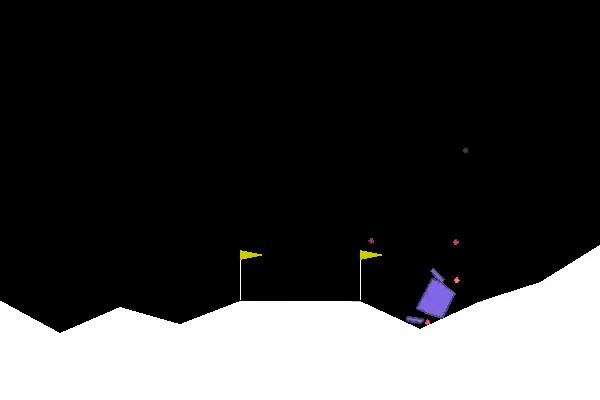
\includegraphics[width=\textwidth/2]
  {diagrams/lunarlander.jpg}
  \caption{Screenshot of "LunarLander-v2"}
\end{figure}

"LunarLander-v2" is a far more complex environment to
master since its action space is higher, it offers far more
different observations and a more complex scoring system.

When we tried to train an agent that would master
"LunarLander-v2" on our development environment we were
never able to build an agent that would succeed in this
(every time we tried running our program we canceled after
four hours of runtime).

We did four test runs on our operational environment (in
room 1.242), each with a different approach either in the
amount of Executors (one or two) or the sanitation done
to the training data (less strict which means more training
data or more strict which means higher qualitiy of the
training data).

For each test we used a neural network with two hidden
layers, both with 64 artificial neurons.
\newline\newline
The test runs:
\begin{enumerate}

  \item This test run was done with a less strict policy
        toward our training data which means we took every
        episode that generated a score of over 0 and
        sanitized the episodes that had a score better than
        -400.

        Sanitation means we normalized every action's
        single score and took only the actions with a score
        better than 0.4 (we thought doing this we could
        cut out the part where the agent loses control over
        the ufo before crashing)

        We had 9 Workers running on 9 different machines
        and one Executor. Every Worker spawned 1 process
        generating training data with the agent and 5
        processes generating training data randomly.

        Every process ran 1000 Episodes.

        This test run was terminated after approximately
        one hour.

        \textbf{Observations:}

        \begin{itemize}

          \item 1000 Episodes were far too small. The
                Workers flooded the data\_queue with
                messages containing only a small amound of
                data.

          \item We discovered a very serious bottleneck.
                The messages containing the training data
                are formatted as a JSON string
                representation of a Python list which is
                parsed back into a list object when the
                Executor's main process receives it.

                But before training the list has to be
                parsed again into a format our agent (cmp.
                \ref{s_agent}) understands. The list
                containing tuples with the observation and
                the corresponding action has to be splitted
                an parsed to a NumPy Array. This parsing is
                very expensive and while doing the parsing
                the Executioner's TTSL process holds the
                shared list object (which means the main
                process has to wait until the TTSL process
                releases the list's mutex, which is one
                reason why the data\_queue was so flooded).

        \end{itemize}

  \item This time we tried to conquer the issues we faced
        in the first test run. We used the same policy
        towards our training data but increased the amount
        of episodes played by each process. Every process
        doing generation randomly now did 10000 episodes
        while the ones using the agent played 5000.

        Also now we spawned 5 processes using the agent and
        5 doing random actions.

        To avoid the bottleneck this time we added another
        Executor which roughly follows a reinforcement
        lerning technique called Double Q-Learing and is
        used to avoid overestimation for the training data
        (the agent doing the same mistakes over and over,
        because it trains with data it generated itself).
        \cite{jonas1}

        Both Executors are in a race condition for the next
        training data and both provide every Worker with
        its agent which we thought would lead to quality
        training data while keeping the data\_queue small.

        We terminated this test run after approximately
        one and three quarters of an hour, after 11
        iterations of the TTSL (both Executors). Both
        Executors combined had over 60 million data points
        and 40GB of more training data was still in the
        data\_queue.

        \textbf{Observations:}

        \begin{itemize}

          \item We only postponed the moment our
                application would kill itself with too much
                training data. Parsing again was too much.

          \item Even though we had 60 million data points
                the agents were not able to show much
                progress. Not many test runs were able to
                exceed -150 (200 being the score an episode
                is played successfully).

        \end{itemize}

  \item After having again the problem of an overflowing
        data\_queue and not much progress even after 11
        iterations we tried a stricter policy. We took only
        episodes which generated a score of over 100 and
        sanitized the episodes which had a score over -50.

        Again we used to Executors and 8 Workers, all on
        different machines.

        We terminated this test run after approximately 45
        minutes, both Executors having more than 16 million
        data points as their training data set.

        \textbf{Observations:}

        \begin{itemize}

          \item At the first iterations we had some more
                success (scores over 100 which we were
                never able to reach before), but, at the
                end, even though the Executors both had
                16 million data points, all on episodes
                with a score that had at least reached -50,
                both agents settled for test results around
                -150, like the two test runs before.

                We were not able to increase the
                performance of our agents.

        \end{itemize}

  \item We increased the strictness even more. We took only
        episodes that generated a score better than 150 and
        cut out the sanitation.

        This time we used only one Executor and again 9
        Workers.

        Again we terminated after approximately 45 minutes,
        again unsuccessful.

        \textbf{Observations:}

        \begin{itemize}

          \item Before the workers can use the agent the
                agent has to be trained with 100 percent
                random generated data. Because the policy
                was so strict the first 6 received
                messages on the data\_queue were empty. The
                seventh received message contained only 427
                data points.

          \item Like the third test run this test run had
                even greater success at the beginning,
                once actually reaching 200. But again, even
                though only training with data better than
                150 the agent settled at -150, only
                occasionally getting a better result around
                -50.

        \end{itemize}

\end{enumerate}

So, while we were able to create a distributed application
that uses a modern approach to concurrency and was able to
crunch a lot of numbers in a small amount of time,
unfortunately we were not able to build an agent that
could master "LunarLander-v2".

\subsection{Where to go, what to do next}

There are some points we would like to add to our
application in order to make it able to build an agent
that is good enough for "LunarLander-v2".

\begin{itemize}[label={}]

  \item \textbf{Statistical methods for data sanitation and
                a better agent:}

        Since we wanted to build an application that
        takes a task that takes a long time if done
        not concurrently and make it fast, we never really
        looked deeper into statistical methods from the
        fields of artificial intelligence research and
        data science that could have helped us build a
        better agent or a better training data set.

        We thought we could generate enough data to
        outweigh the weaknesses our project shows when it
        comes to optimization of agent or training data
        set.

        In the end our approach failed, so maybe by adding
        some optimizations of the agent or the training
        data set the application could be able to produce
        an agent that is able to succeed.

  \item \textbf{Some sort of load balancing:}

        We had hughe troubles in two test cases with
        an overflowing data\_queue.

        Our static approach (playing the same amount of
        episodes every iteration of the GSL (cmp.
        \ref{s_worker}) did not work that well. At some
        time the Workers start to overwhelm the
        Executor(s).

        To avoid this a unit doing load balancing should be
        added to the application that supervises the
        training data set generation using meta data from
        the Executor and the RabbitMQ.

  \item \textbf{Doing something with the parsing
                bottlneck of the Executor:}

        The parsing of the training data took longer than
        the actual training (optimized by Tensorflow).

        Right now the parsing is done in a single process
        (the TTSL process (cmp. \ref{s_executor})), however
        we think the parsing could be optimized using
        a concurrent approach (e.g. worker processes like
        we use for the data generation (cmp.
        \ref{s_worker})).

  \item \textbf{Optimize the protocolling unit:}

        The problem with our current protocolling unit is,
        that it only saves the protocol when the program
        is finished successfully, which does not help when
        failing (like we did).

        The protocolling unit should safe the data more
        often (e.g. could be integrated in the TTSL process
        (cmp. \ref{s_executor}) or a new process only for
        protocolling could be spawned).

\end{itemize}


\printindex
\Urlmuskip 0mu plus 1mu\relax
\bibliography{wpfvs_bib}
\end{document}
